% AUTO-GENERATED vector figure (scratch build_vector_canvases.py). Vector text +
% full-resolution embedded photos + per-panel arXiv hyperlink & verified figure number.
\begin{figure*}[tp]
\centering
\resizebox{\textwidth}{!}{%
\begin{tikzpicture}[x=1cm,y=1cm]
\definecolor{c7A2438}{HTML}{7A2438}
\definecolor{c1F6F8B}{HTML}{1F6F8B}
\definecolor{c5B3A8A}{HTML}{5B3A8A}
\fill[black!88] (0,0) rectangle (13.800,-0.580);
\node[anchor=west,text=white,font=\small\bfseries,inner sep=0] at (0.14,-0.290) {Results reported across the surveyed systems};
\node[anchor=east,text=white!60,font=\scriptsize,inner sep=0] at (13.660,-0.290) {vector, zoomable, per-panel arXiv links};
\fill[c7A2438] (0,-0.580) rectangle (13.800,-1.080);
\node[anchor=west,text=white,font=\footnotesize\bfseries,inner sep=0] at (0.14,-0.830) {Success-rate and ablation bar charts};
\node[anchor=north west,inner sep=0] at (0.070,-1.150) {\href{https://arxiv.org/abs/2307.15818}{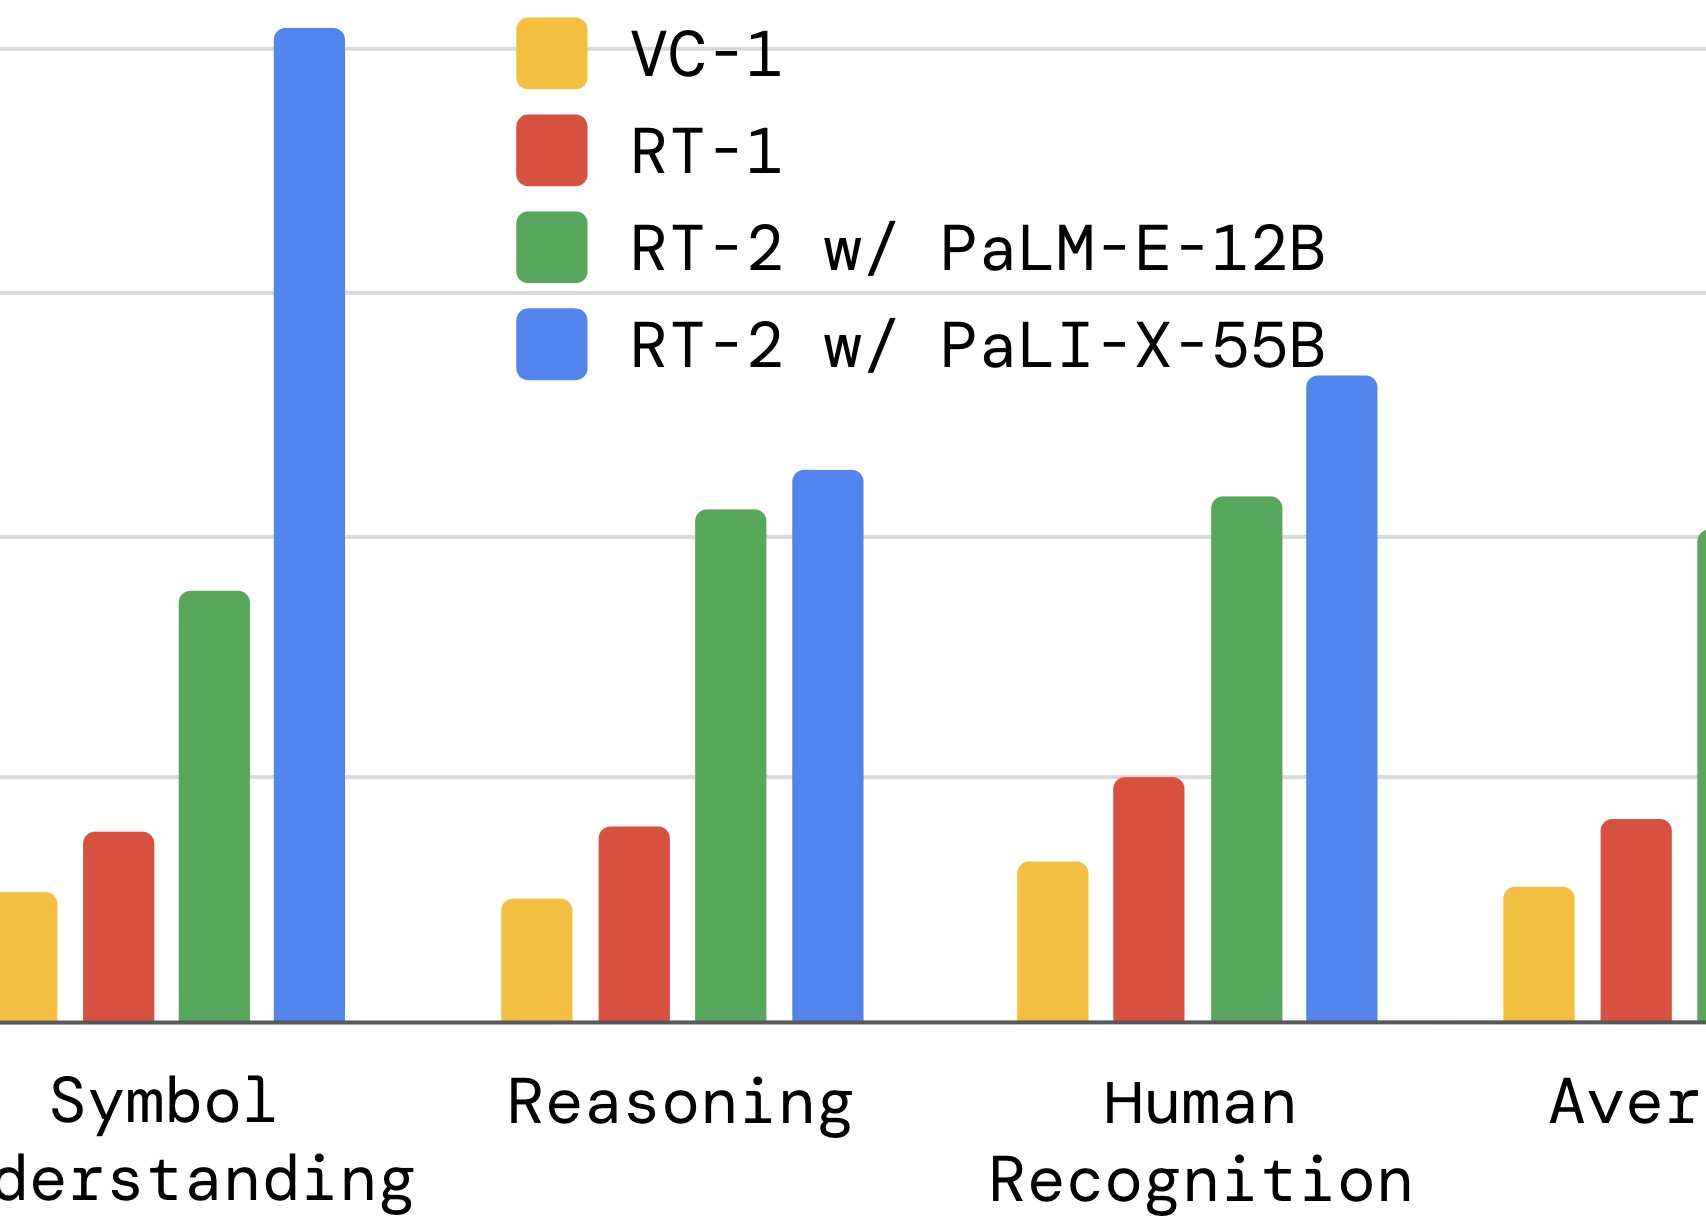
\includegraphics[width=1.891cm]{figures/img/canvas_tiles/plt_306.jpg}}};
\draw[black!35,line width=0.35pt] (0.070,-1.150) rectangle (1.961,-2.512);
\node[anchor=north west,text=ACMDarkBlue,font=\tiny\bfseries,inner sep=0] at (0.100,-2.542) {\href{https://arxiv.org/abs/2307.15818}{RT-2}};
\node[anchor=north west,text=black!60,font=\tiny,inner sep=0] at (0.100,-2.747) {\href{https://arxiv.org/abs/2307.15818}{Fig.\,6a~p.10}};
\node[anchor=north west,inner sep=0] at (2.031,-1.150) {\href{https://arxiv.org/abs/2209.07753}{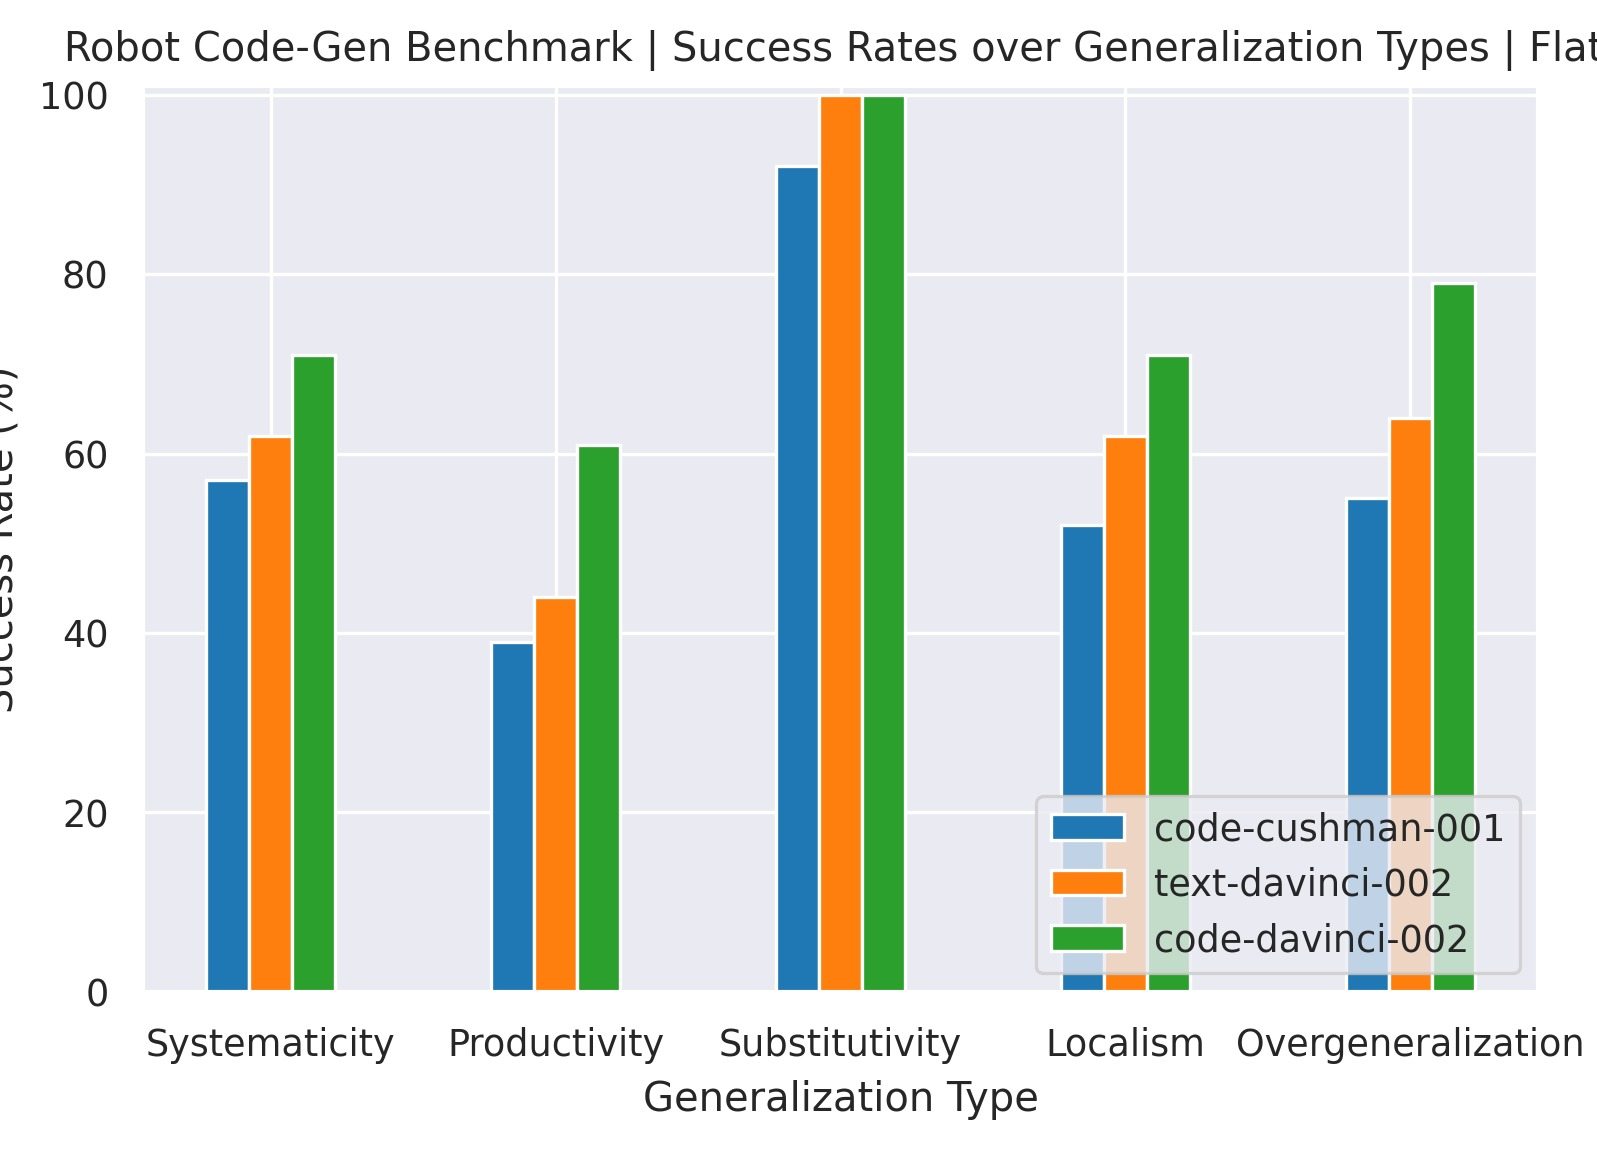
\includegraphics[width=1.891cm]{figures/img/canvas_tiles/plt_45.jpg}}};
\draw[black!35,line width=0.35pt] (2.031,-1.150) rectangle (3.923,-2.512);
\node[anchor=north west,text=ACMDarkBlue,font=\tiny\bfseries,inner sep=0] at (2.061,-2.542) {\href{https://arxiv.org/abs/2209.07753}{Code-as-Policies}};
\node[anchor=north west,text=black!60,font=\tiny,inner sep=0] at (2.061,-2.747) {\href{https://arxiv.org/abs/2209.07753}{Fig.\,4~p.11}};
\node[anchor=north west,inner sep=0] at (3.993,-1.150) {\href{https://arxiv.org/abs/2305.16744}{\includegraphics[width=1.891cm]{figures/img/canvas_tiles/plt_64.jpg}}};
\draw[black!35,line width=0.35pt] (3.993,-1.150) rectangle (5.884,-2.512);
\node[anchor=north west,text=ACMDarkBlue,font=\tiny\bfseries,inner sep=0] at (4.023,-2.542) {\href{https://arxiv.org/abs/2305.16744}{Demo2Code}};
\node[anchor=north west,text=black!60,font=\tiny,inner sep=0] at (4.023,-2.747) {\href{https://arxiv.org/abs/2305.16744}{Fig.\,13~p.40}};
\node[anchor=north west,inner sep=0] at (5.954,-1.150) {\href{https://arxiv.org/abs/2310.12931}{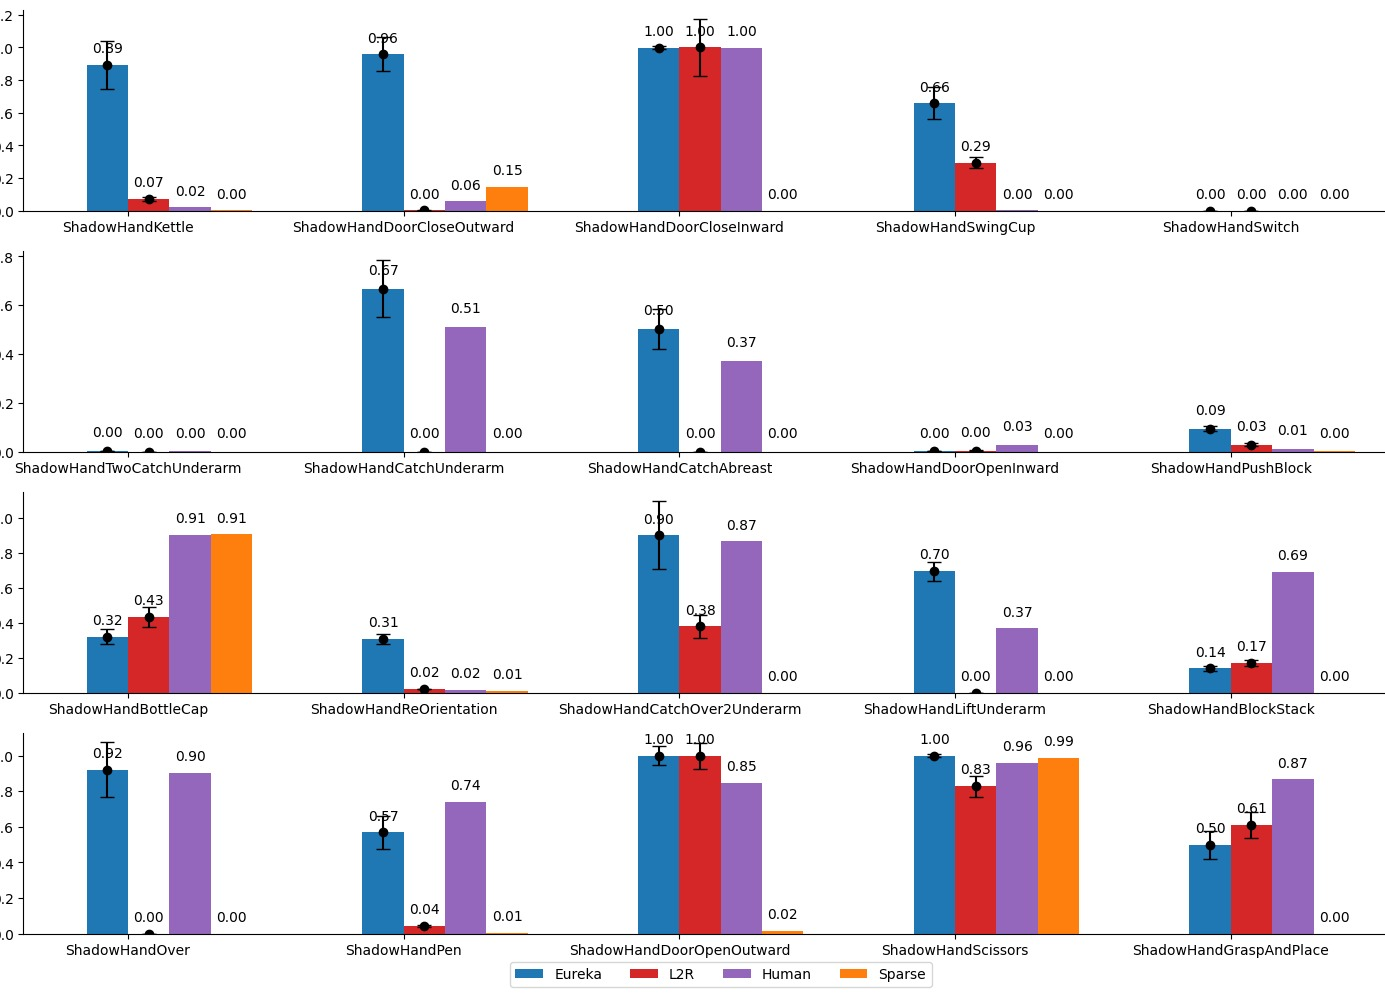
\includegraphics[width=1.891cm]{figures/img/canvas_tiles/plt_96.jpg}}};
\draw[black!35,line width=0.35pt] (5.954,-1.150) rectangle (7.846,-2.512);
\node[anchor=north west,text=ACMDarkBlue,font=\tiny\bfseries,inner sep=0] at (5.984,-2.542) {\href{https://arxiv.org/abs/2310.12931}{Eureka}};
\node[anchor=north west,text=black!60,font=\tiny,inner sep=0] at (5.984,-2.747) {\href{https://arxiv.org/abs/2310.12931}{Fig.\,13~p.29}};
\node[anchor=north west,inner sep=0] at (7.916,-1.150) {\href{https://arxiv.org/abs/2402.14623}{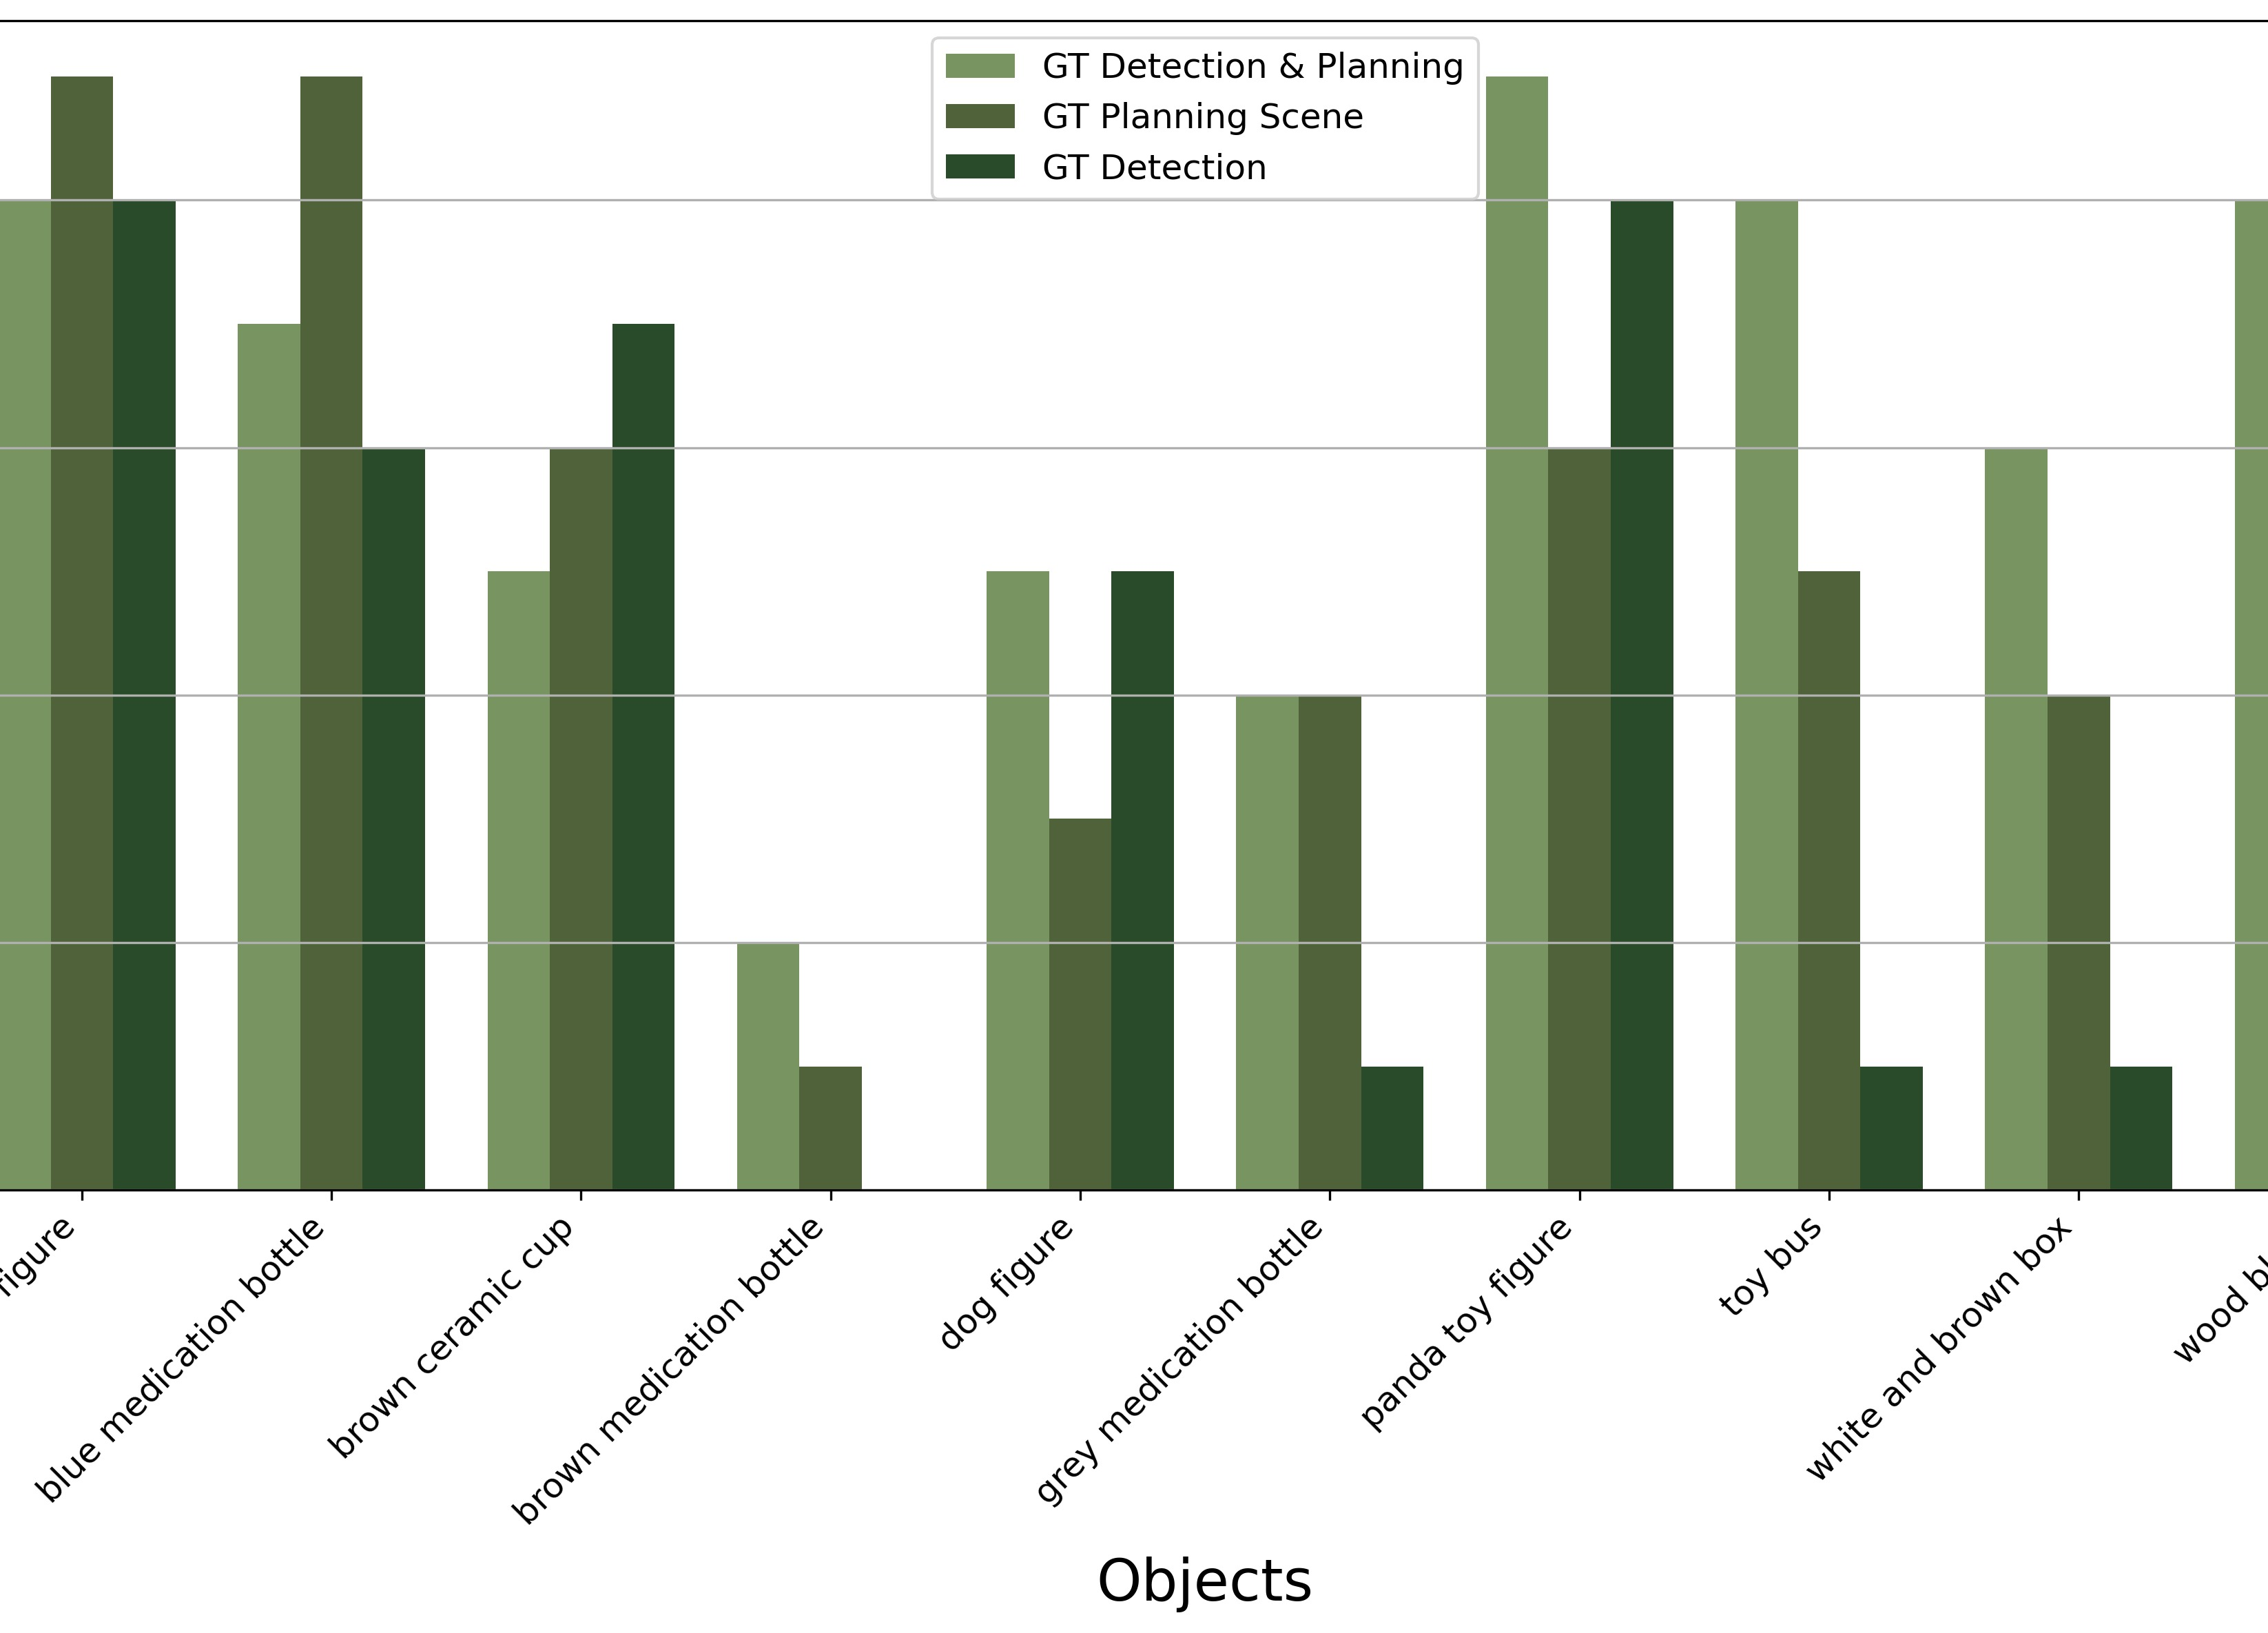
\includegraphics[width=1.891cm]{figures/img/canvas_tiles/plt_284.jpg}}};
\draw[black!35,line width=0.35pt] (7.916,-1.150) rectangle (9.807,-2.512);
\node[anchor=north west,text=ACMDarkBlue,font=\tiny\bfseries,inner sep=0] at (7.946,-2.542) {\href{https://arxiv.org/abs/2402.14623}{RoboScript}};
\node[anchor=north west,text=black!60,font=\tiny,inner sep=0] at (7.946,-2.747) {\href{https://arxiv.org/abs/2402.14623}{Fig.\,8~p.10}};
\node[anchor=north west,inner sep=0] at (9.877,-1.150) {\href{https://arxiv.org/abs/2410.24164}{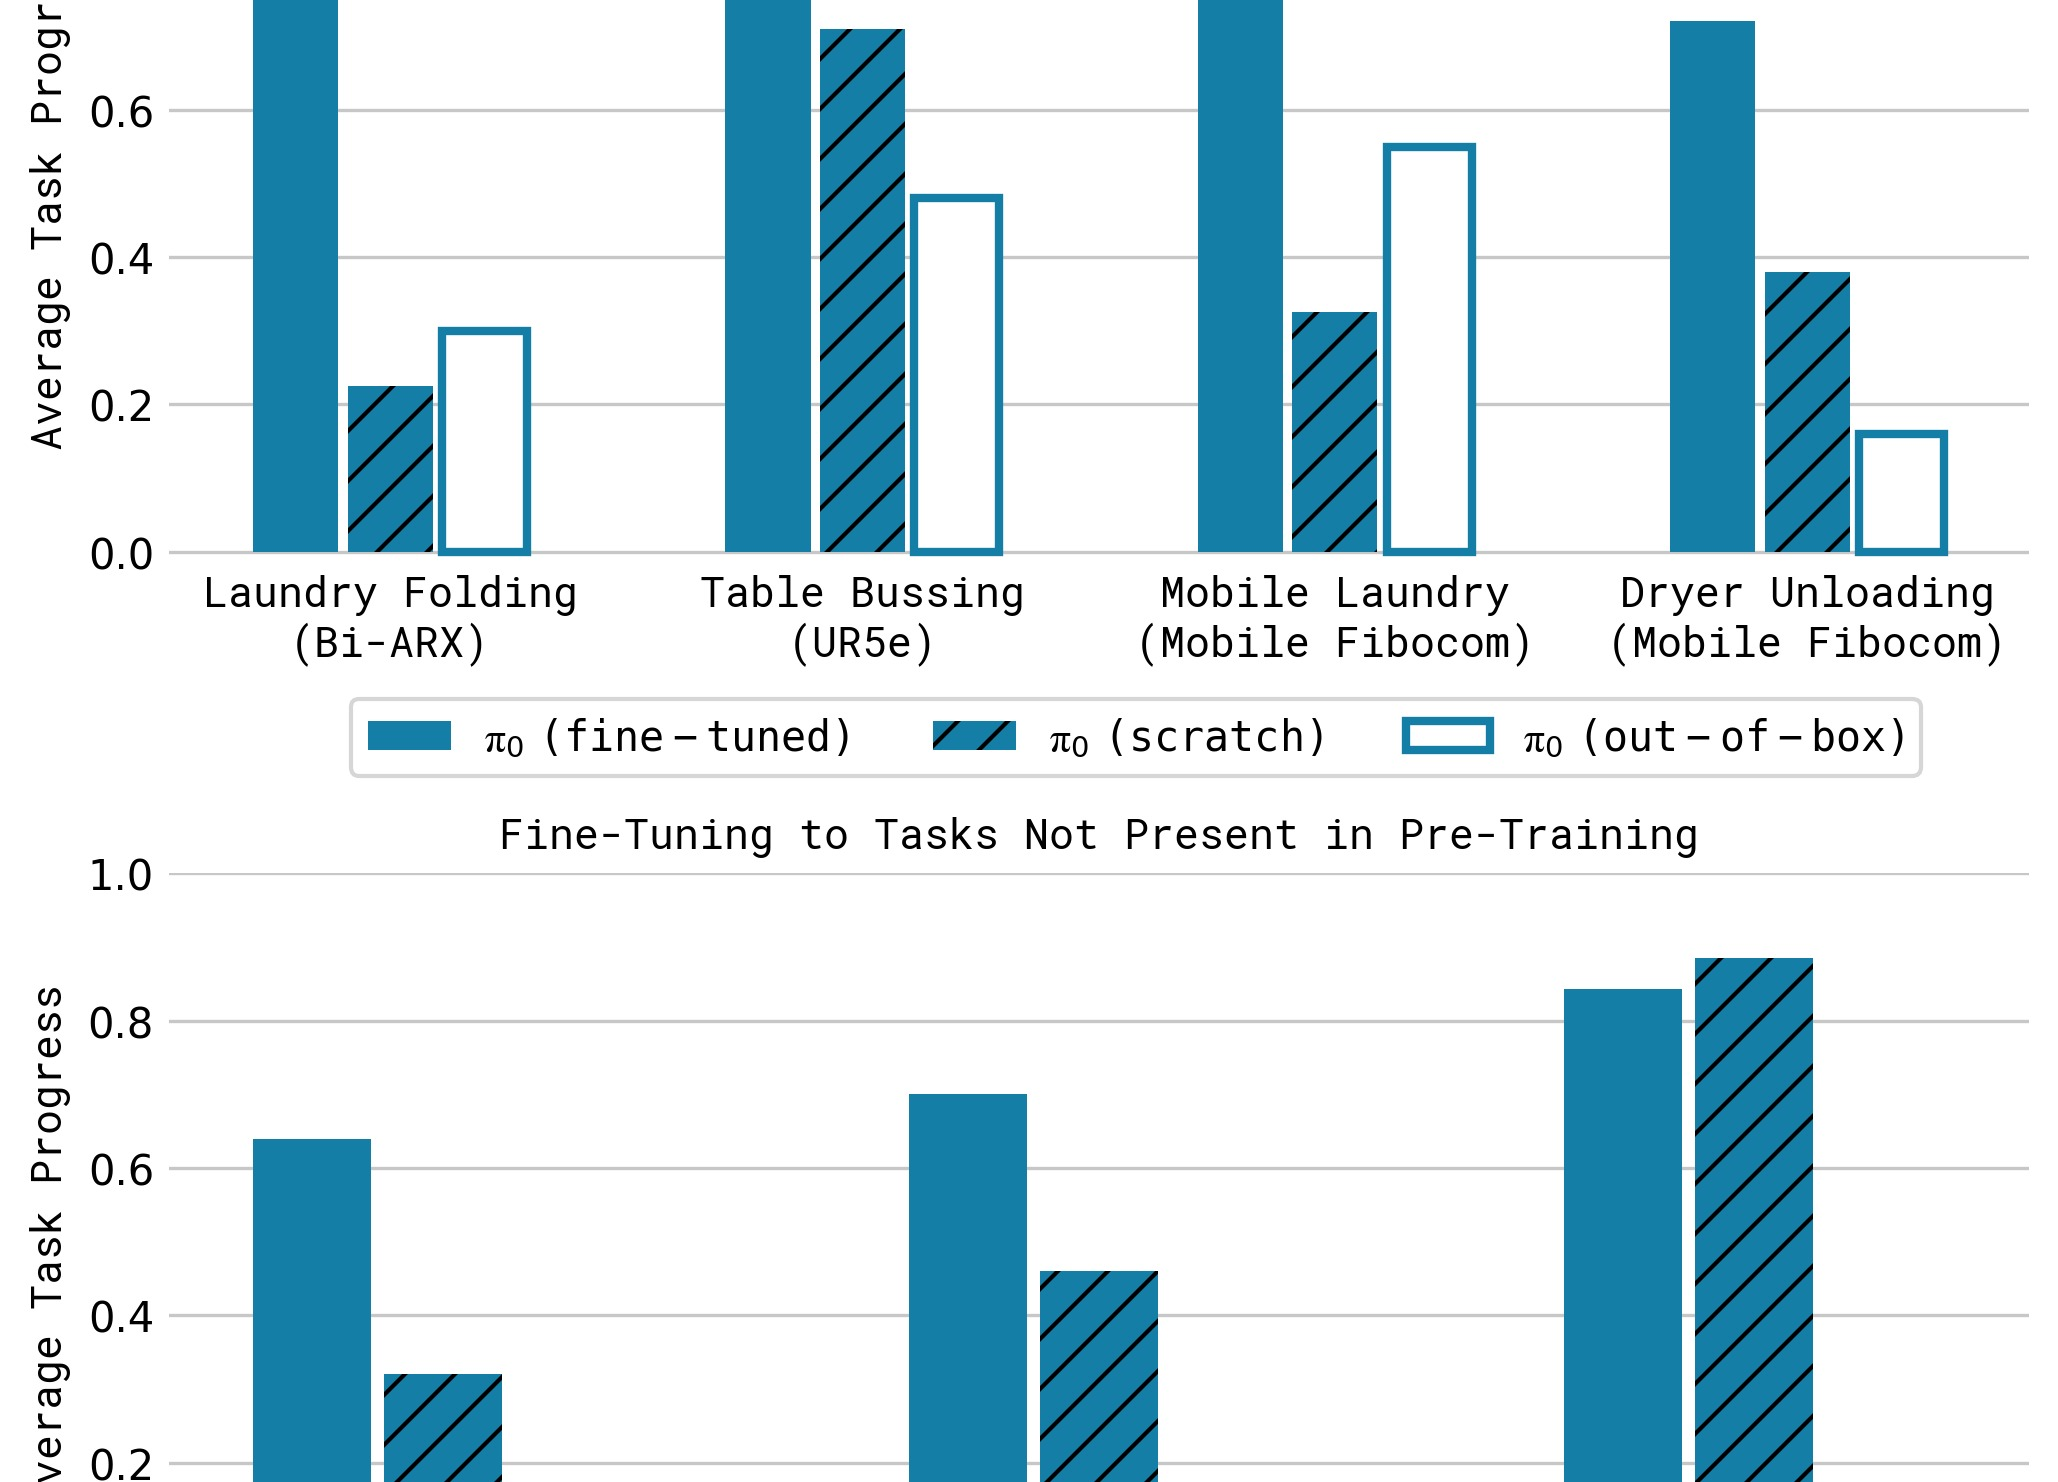
\includegraphics[width=1.891cm]{figures/img/canvas_tiles/plt_217.jpg}}};
\draw[black!35,line width=0.35pt] (9.877,-1.150) rectangle (11.769,-2.512);
\node[anchor=north west,text=ACMDarkBlue,font=\tiny\bfseries,inner sep=0] at (9.907,-2.542) {\href{https://arxiv.org/abs/2410.24164}{Pi-0}};
\node[anchor=north west,text=black!60,font=\tiny,inner sep=0] at (9.907,-2.747) {\href{https://arxiv.org/abs/2410.24164}{Fig.\,13~p.11}};
\node[anchor=north west,inner sep=0] at (11.839,-1.150) {\href{https://arxiv.org/abs/2303.12153}{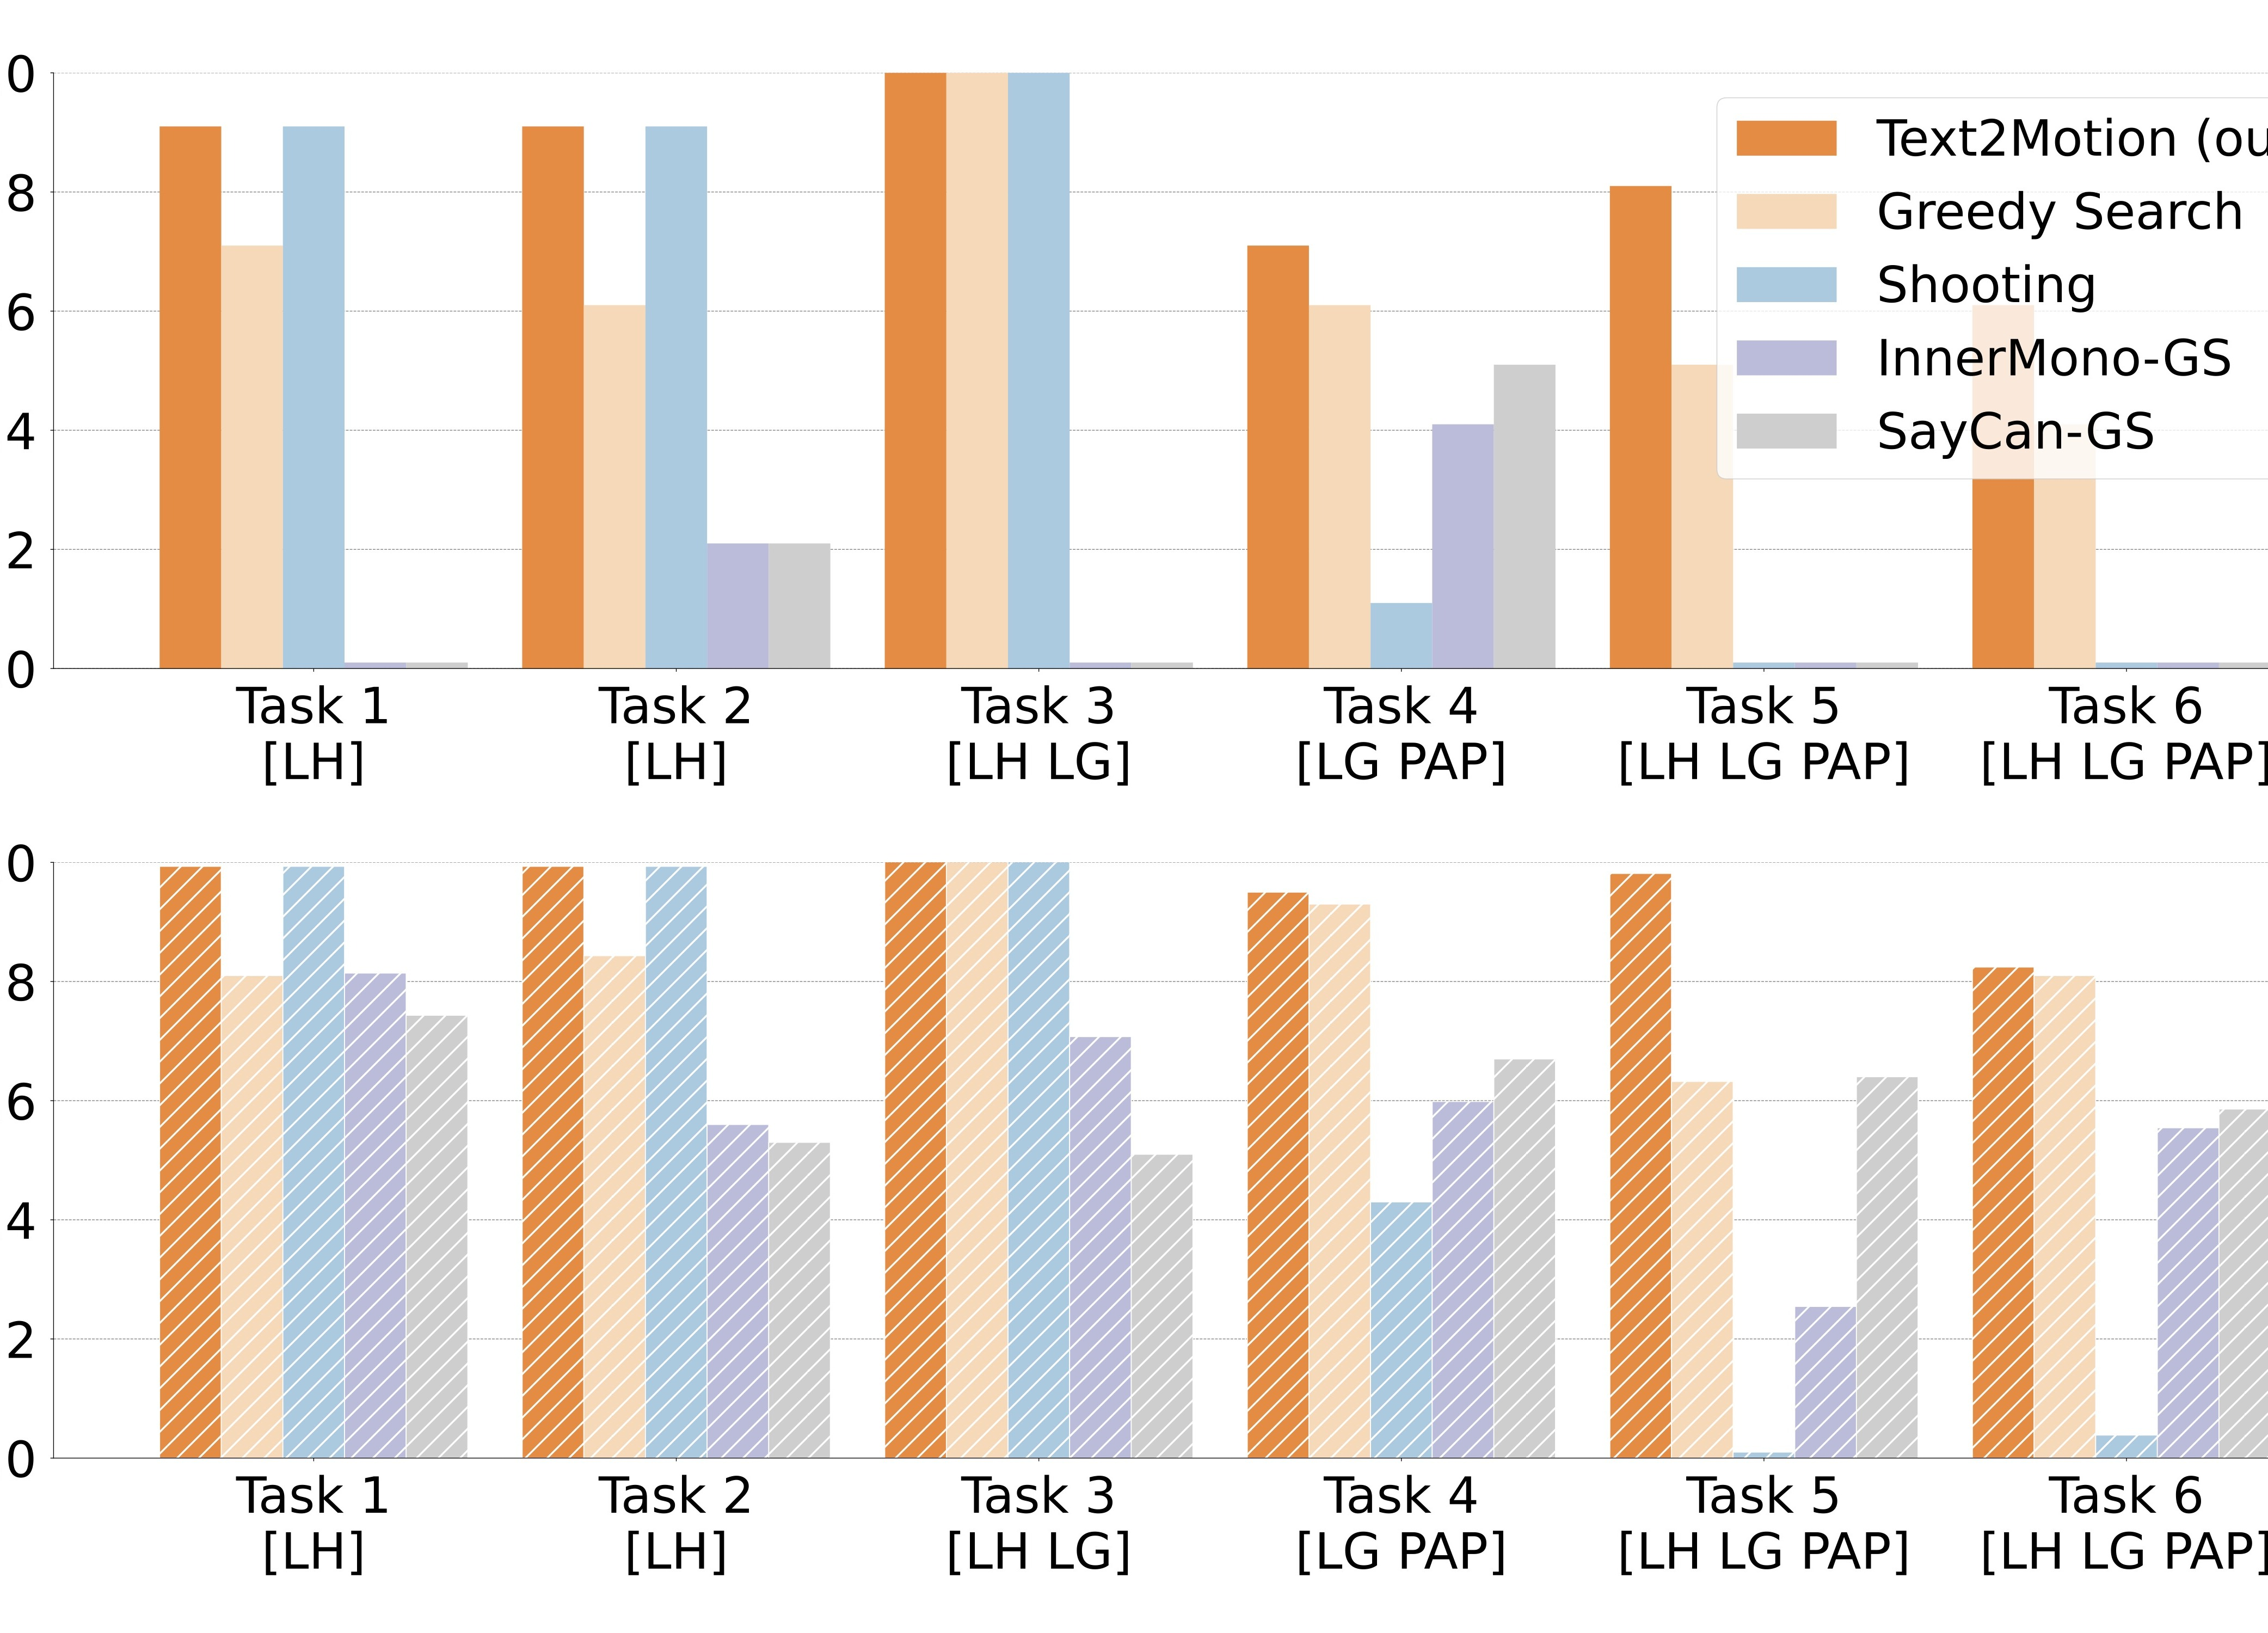
\includegraphics[width=1.891cm]{figures/img/canvas_tiles/plt_333.jpg}}};
\draw[black!35,line width=0.35pt] (11.839,-1.150) rectangle (13.730,-2.512);
\node[anchor=north west,text=ACMDarkBlue,font=\tiny\bfseries,inner sep=0] at (11.869,-2.542) {\href{https://arxiv.org/abs/2303.12153}{Text2Motion}};
\node[anchor=north west,text=black!60,font=\tiny,inner sep=0] at (11.869,-2.747) {\href{https://arxiv.org/abs/2303.12153}{Fig.\,5~p.10}};
\fill[c1F6F8B] (0,-3.002) rectangle (13.800,-3.502);
\node[anchor=west,text=white,font=\footnotesize\bfseries,inner sep=0] at (0.14,-3.252) {Training and scaling curves};
\node[anchor=north west,inner sep=0] at (0.070,-3.572) {\href{https://arxiv.org/abs/2406.01967}{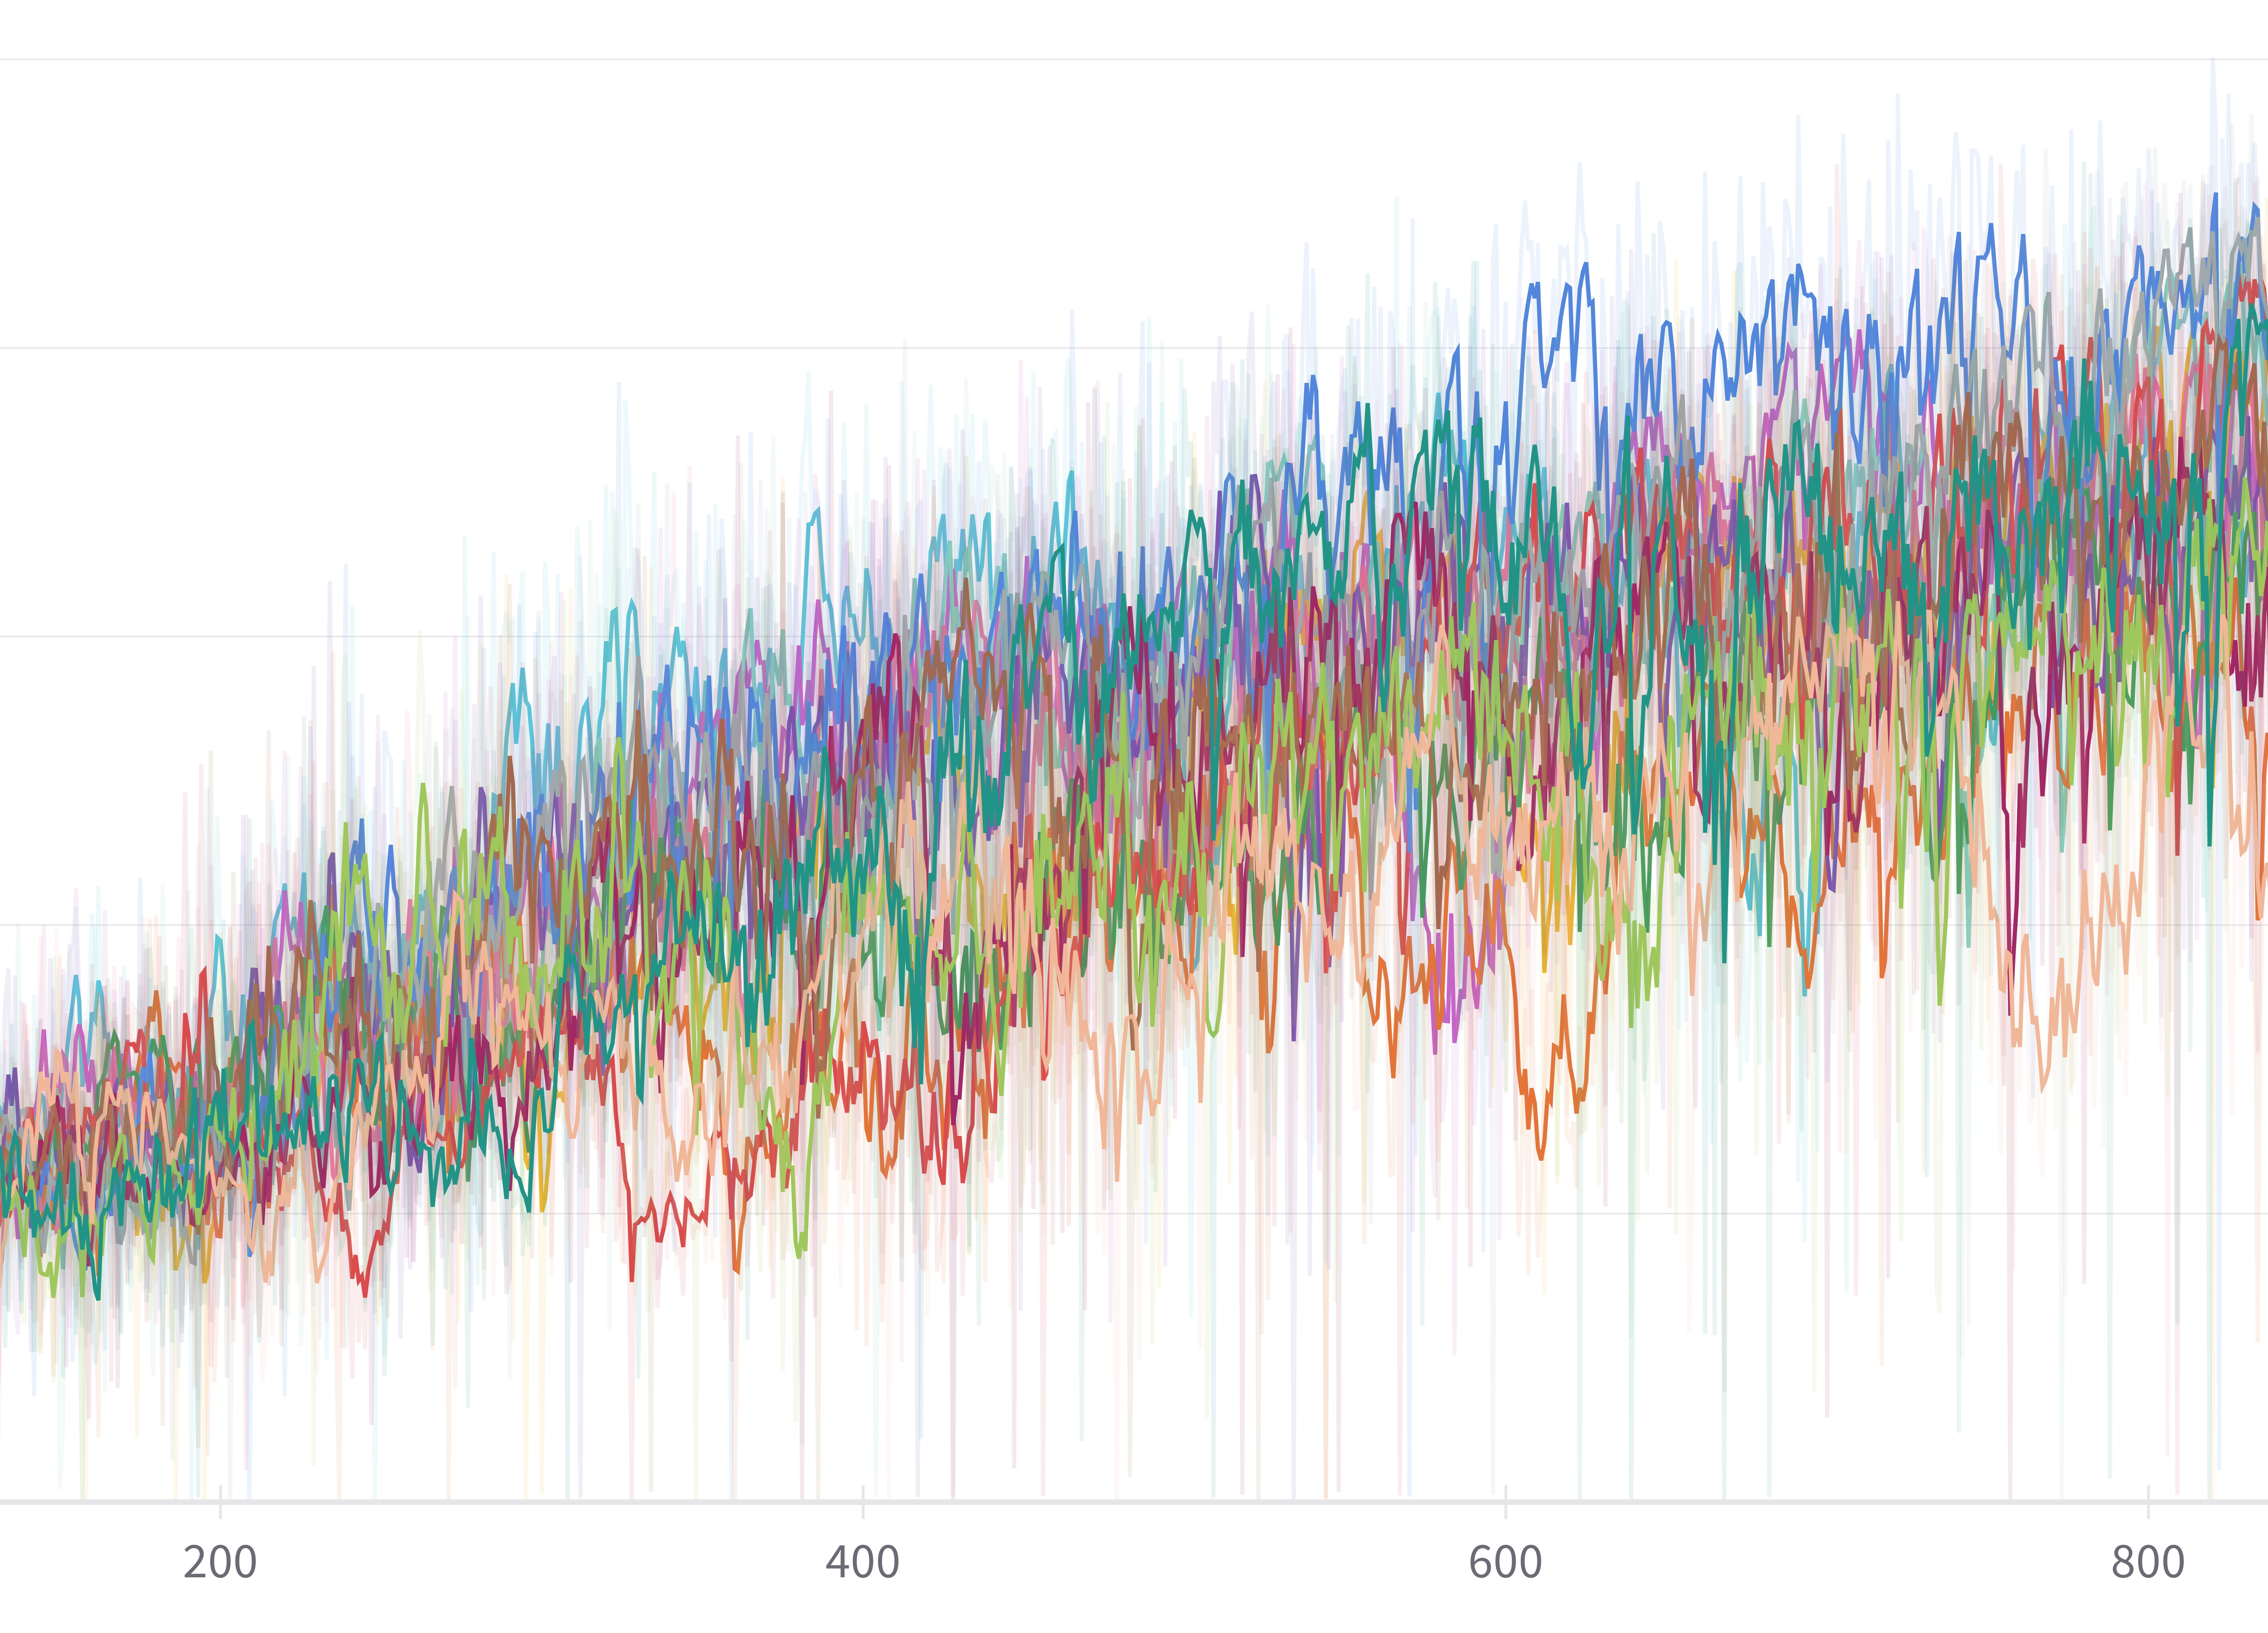
\includegraphics[width=1.891cm]{figures/img/canvas_tiles/plt_80.jpg}}};
\draw[black!35,line width=0.35pt] (0.070,-3.572) rectangle (1.961,-4.934);
\node[anchor=north west,text=ACMDarkBlue,font=\tiny\bfseries,inner sep=0] at (0.100,-4.964) {\href{https://arxiv.org/abs/2406.01967}{DrEureka}};
\node[anchor=north west,text=black!60,font=\tiny,inner sep=0] at (0.100,-5.169) {\href{https://arxiv.org/abs/2406.01967}{Fig.\,8~p.21}};
\node[anchor=north west,inner sep=0] at (2.031,-3.572) {\href{https://arxiv.org/abs/2310.12931}{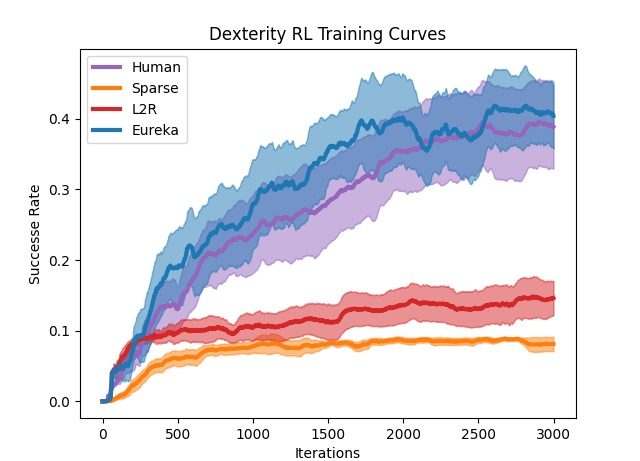
\includegraphics[width=1.891cm]{figures/img/canvas_tiles/plt_95.jpg}}};
\draw[black!35,line width=0.35pt] (2.031,-3.572) rectangle (3.923,-4.934);
\node[anchor=north west,text=ACMDarkBlue,font=\tiny\bfseries,inner sep=0] at (2.061,-4.964) {\href{https://arxiv.org/abs/2310.12931}{Eureka}};
\node[anchor=north west,text=black!60,font=\tiny,inner sep=0] at (2.061,-5.169) {\href{https://arxiv.org/abs/2310.12931}{Fig.\,10~p.28}};
\node[anchor=north west,inner sep=0] at (3.993,-3.572) {\href{https://arxiv.org/abs/2302.04659}{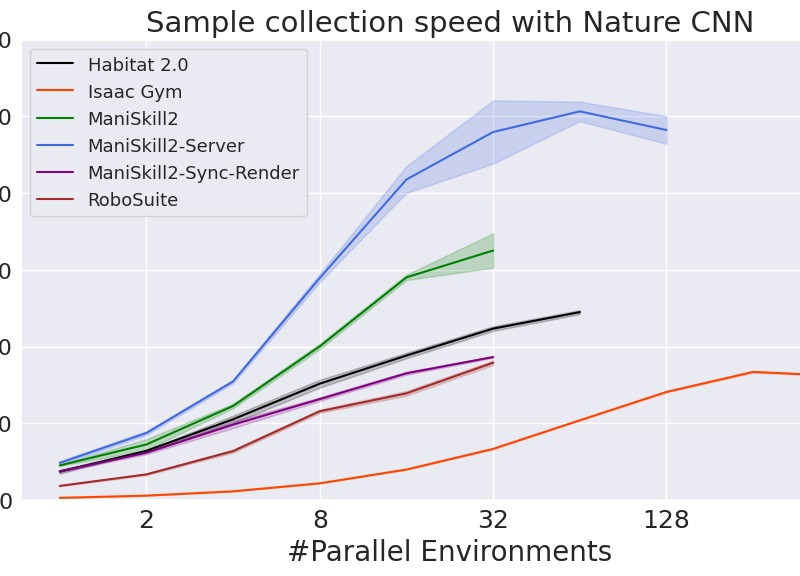
\includegraphics[width=1.891cm]{figures/img/canvas_tiles/plt_171.jpg}}};
\draw[black!35,line width=0.35pt] (3.993,-3.572) rectangle (5.884,-4.934);
\node[anchor=north west,text=ACMDarkBlue,font=\tiny\bfseries,inner sep=0] at (4.023,-4.964) {\href{https://arxiv.org/abs/2302.04659}{ManiSkill2}};
\node[anchor=north west,text=black!60,font=\tiny,inner sep=0] at (4.023,-5.169) {\href{https://arxiv.org/abs/2302.04659}{Fig.\,3~p.7}};
\node[anchor=north west,inner sep=0] at (5.954,-3.572) {\href{https://arxiv.org/abs/2504.16054}{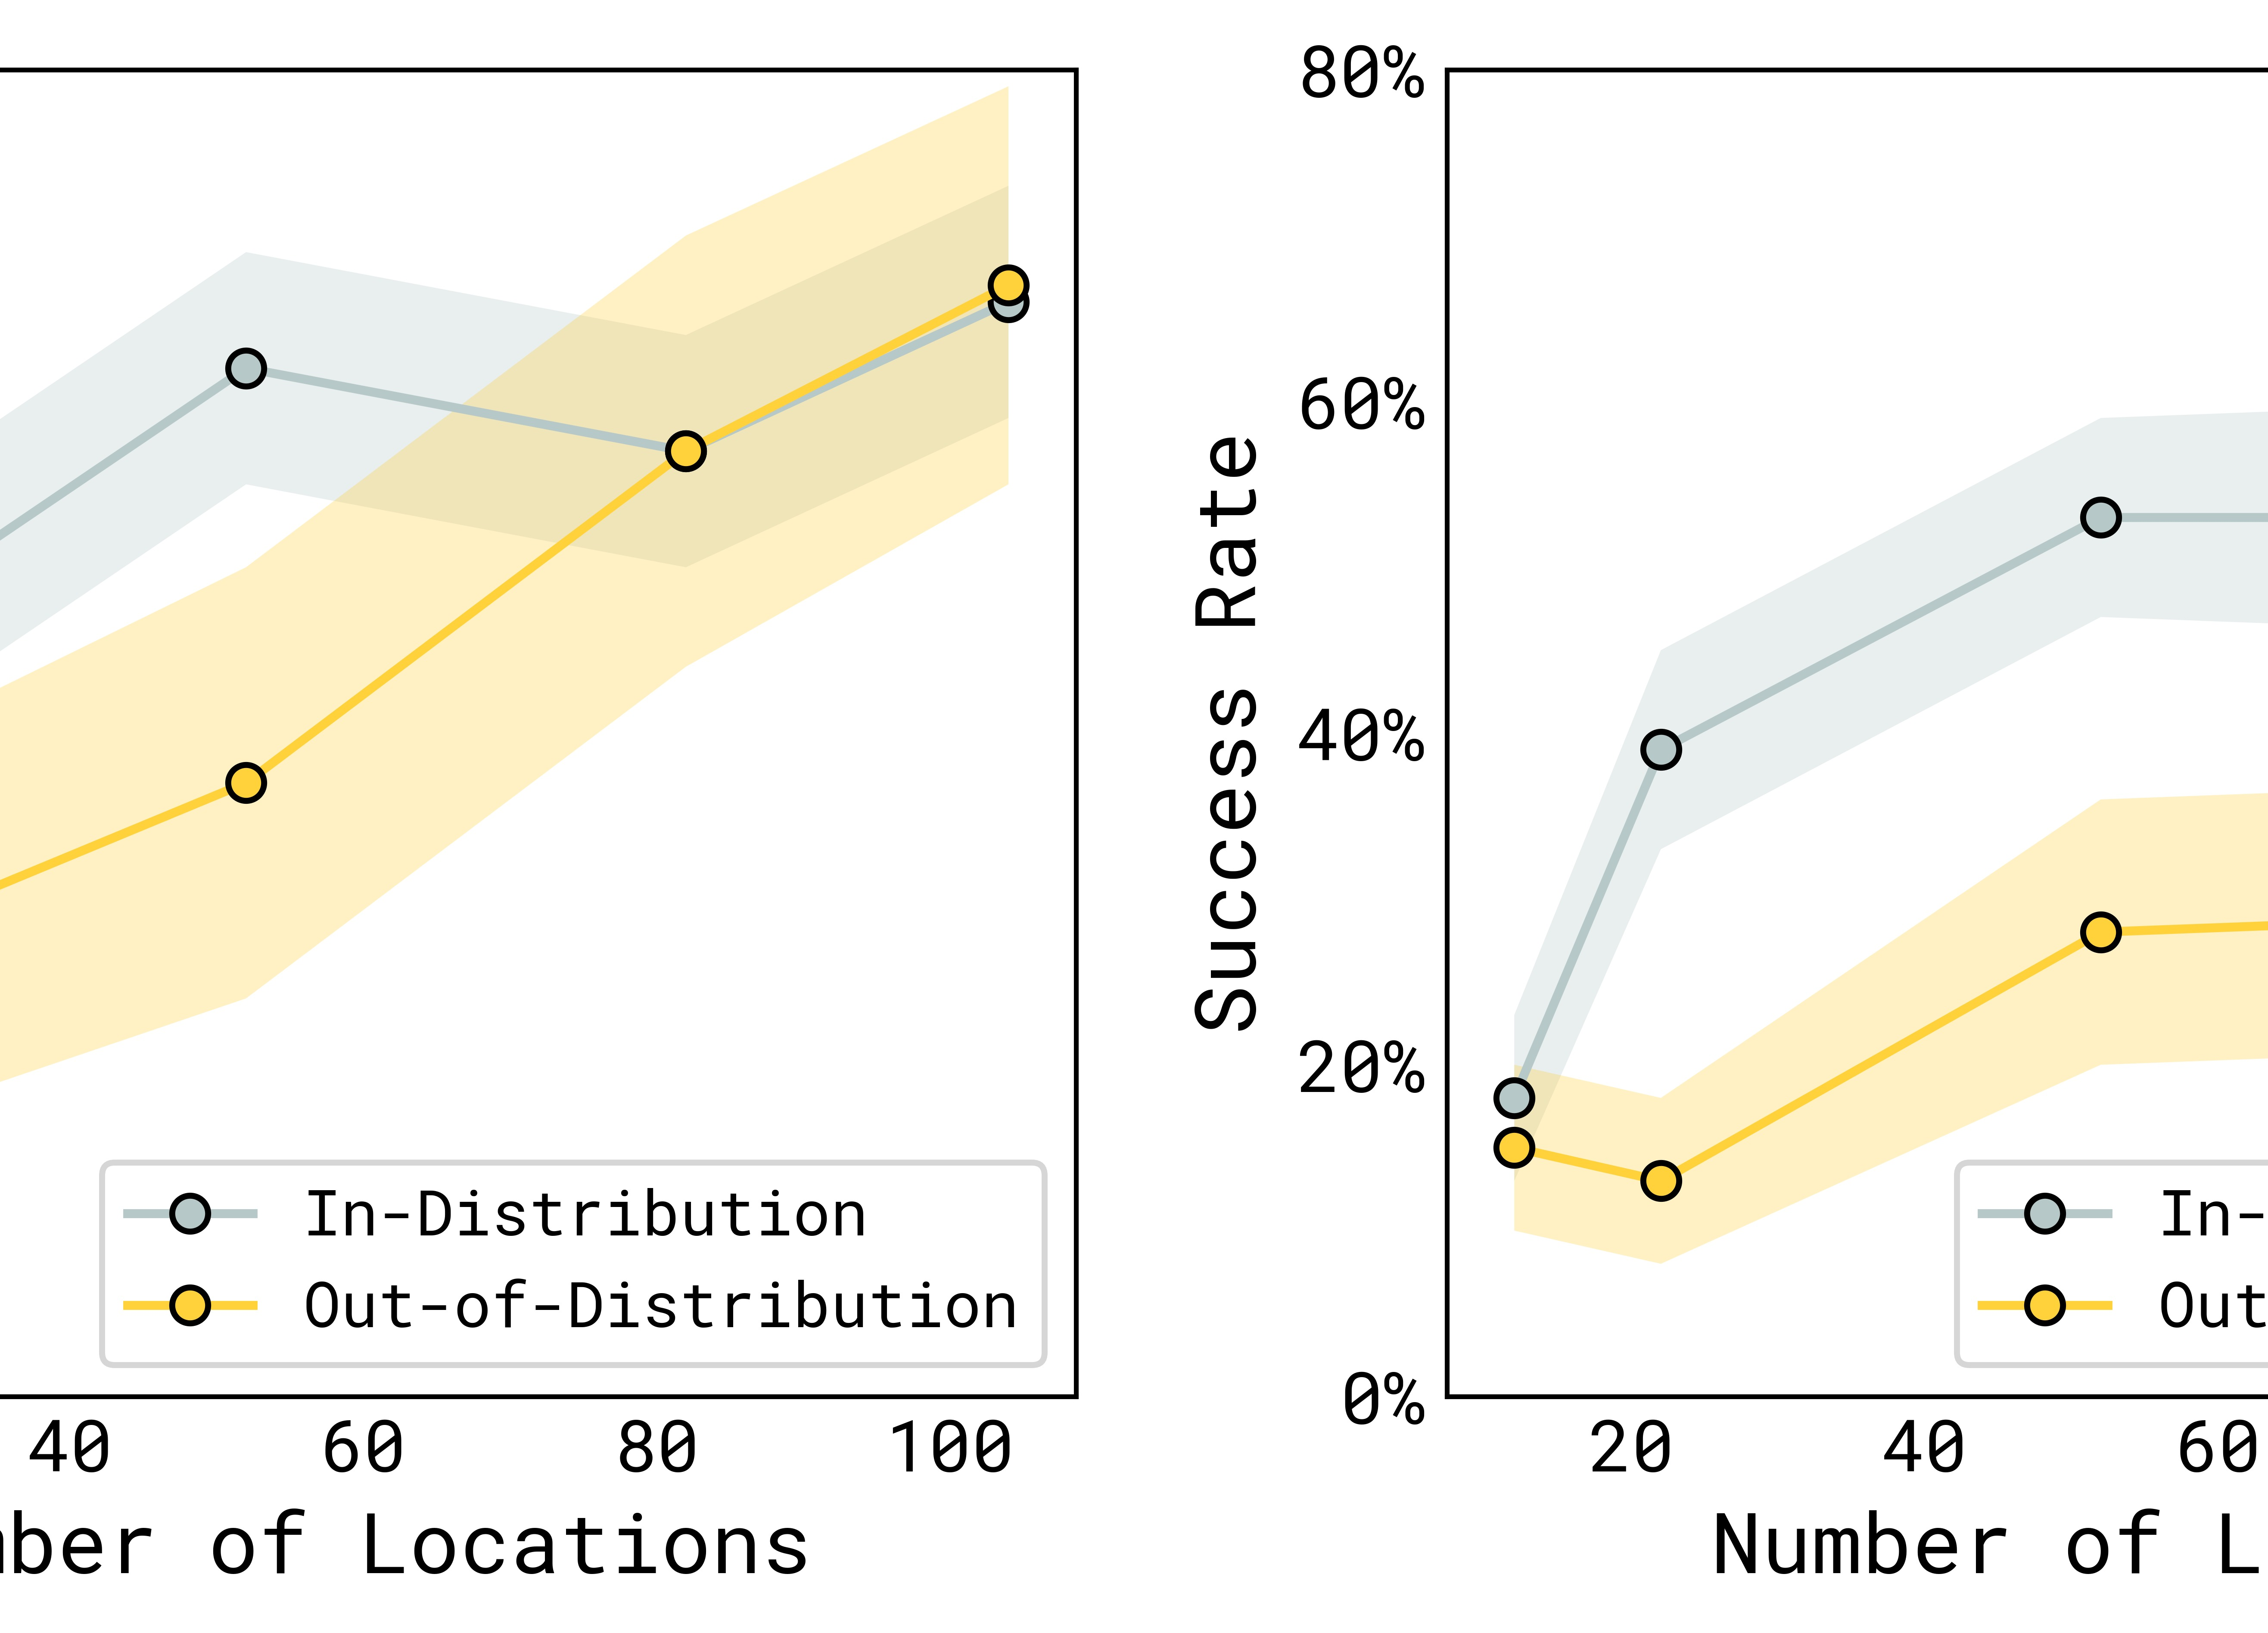
\includegraphics[width=1.891cm]{figures/img/canvas_tiles/plt_221.jpg}}};
\draw[black!35,line width=0.35pt] (5.954,-3.572) rectangle (7.846,-4.934);
\node[anchor=north west,text=ACMDarkBlue,font=\tiny\bfseries,inner sep=0] at (5.984,-4.964) {\href{https://arxiv.org/abs/2504.16054}{Pi-0.5}};
\node[anchor=north west,text=black!60,font=\tiny,inner sep=0] at (5.984,-5.169) {\href{https://arxiv.org/abs/2504.16054}{Fig.\,9~p.9}};
\node[anchor=north west,inner sep=0] at (7.916,-3.572) {\href{https://arxiv.org/abs/2305.16291}{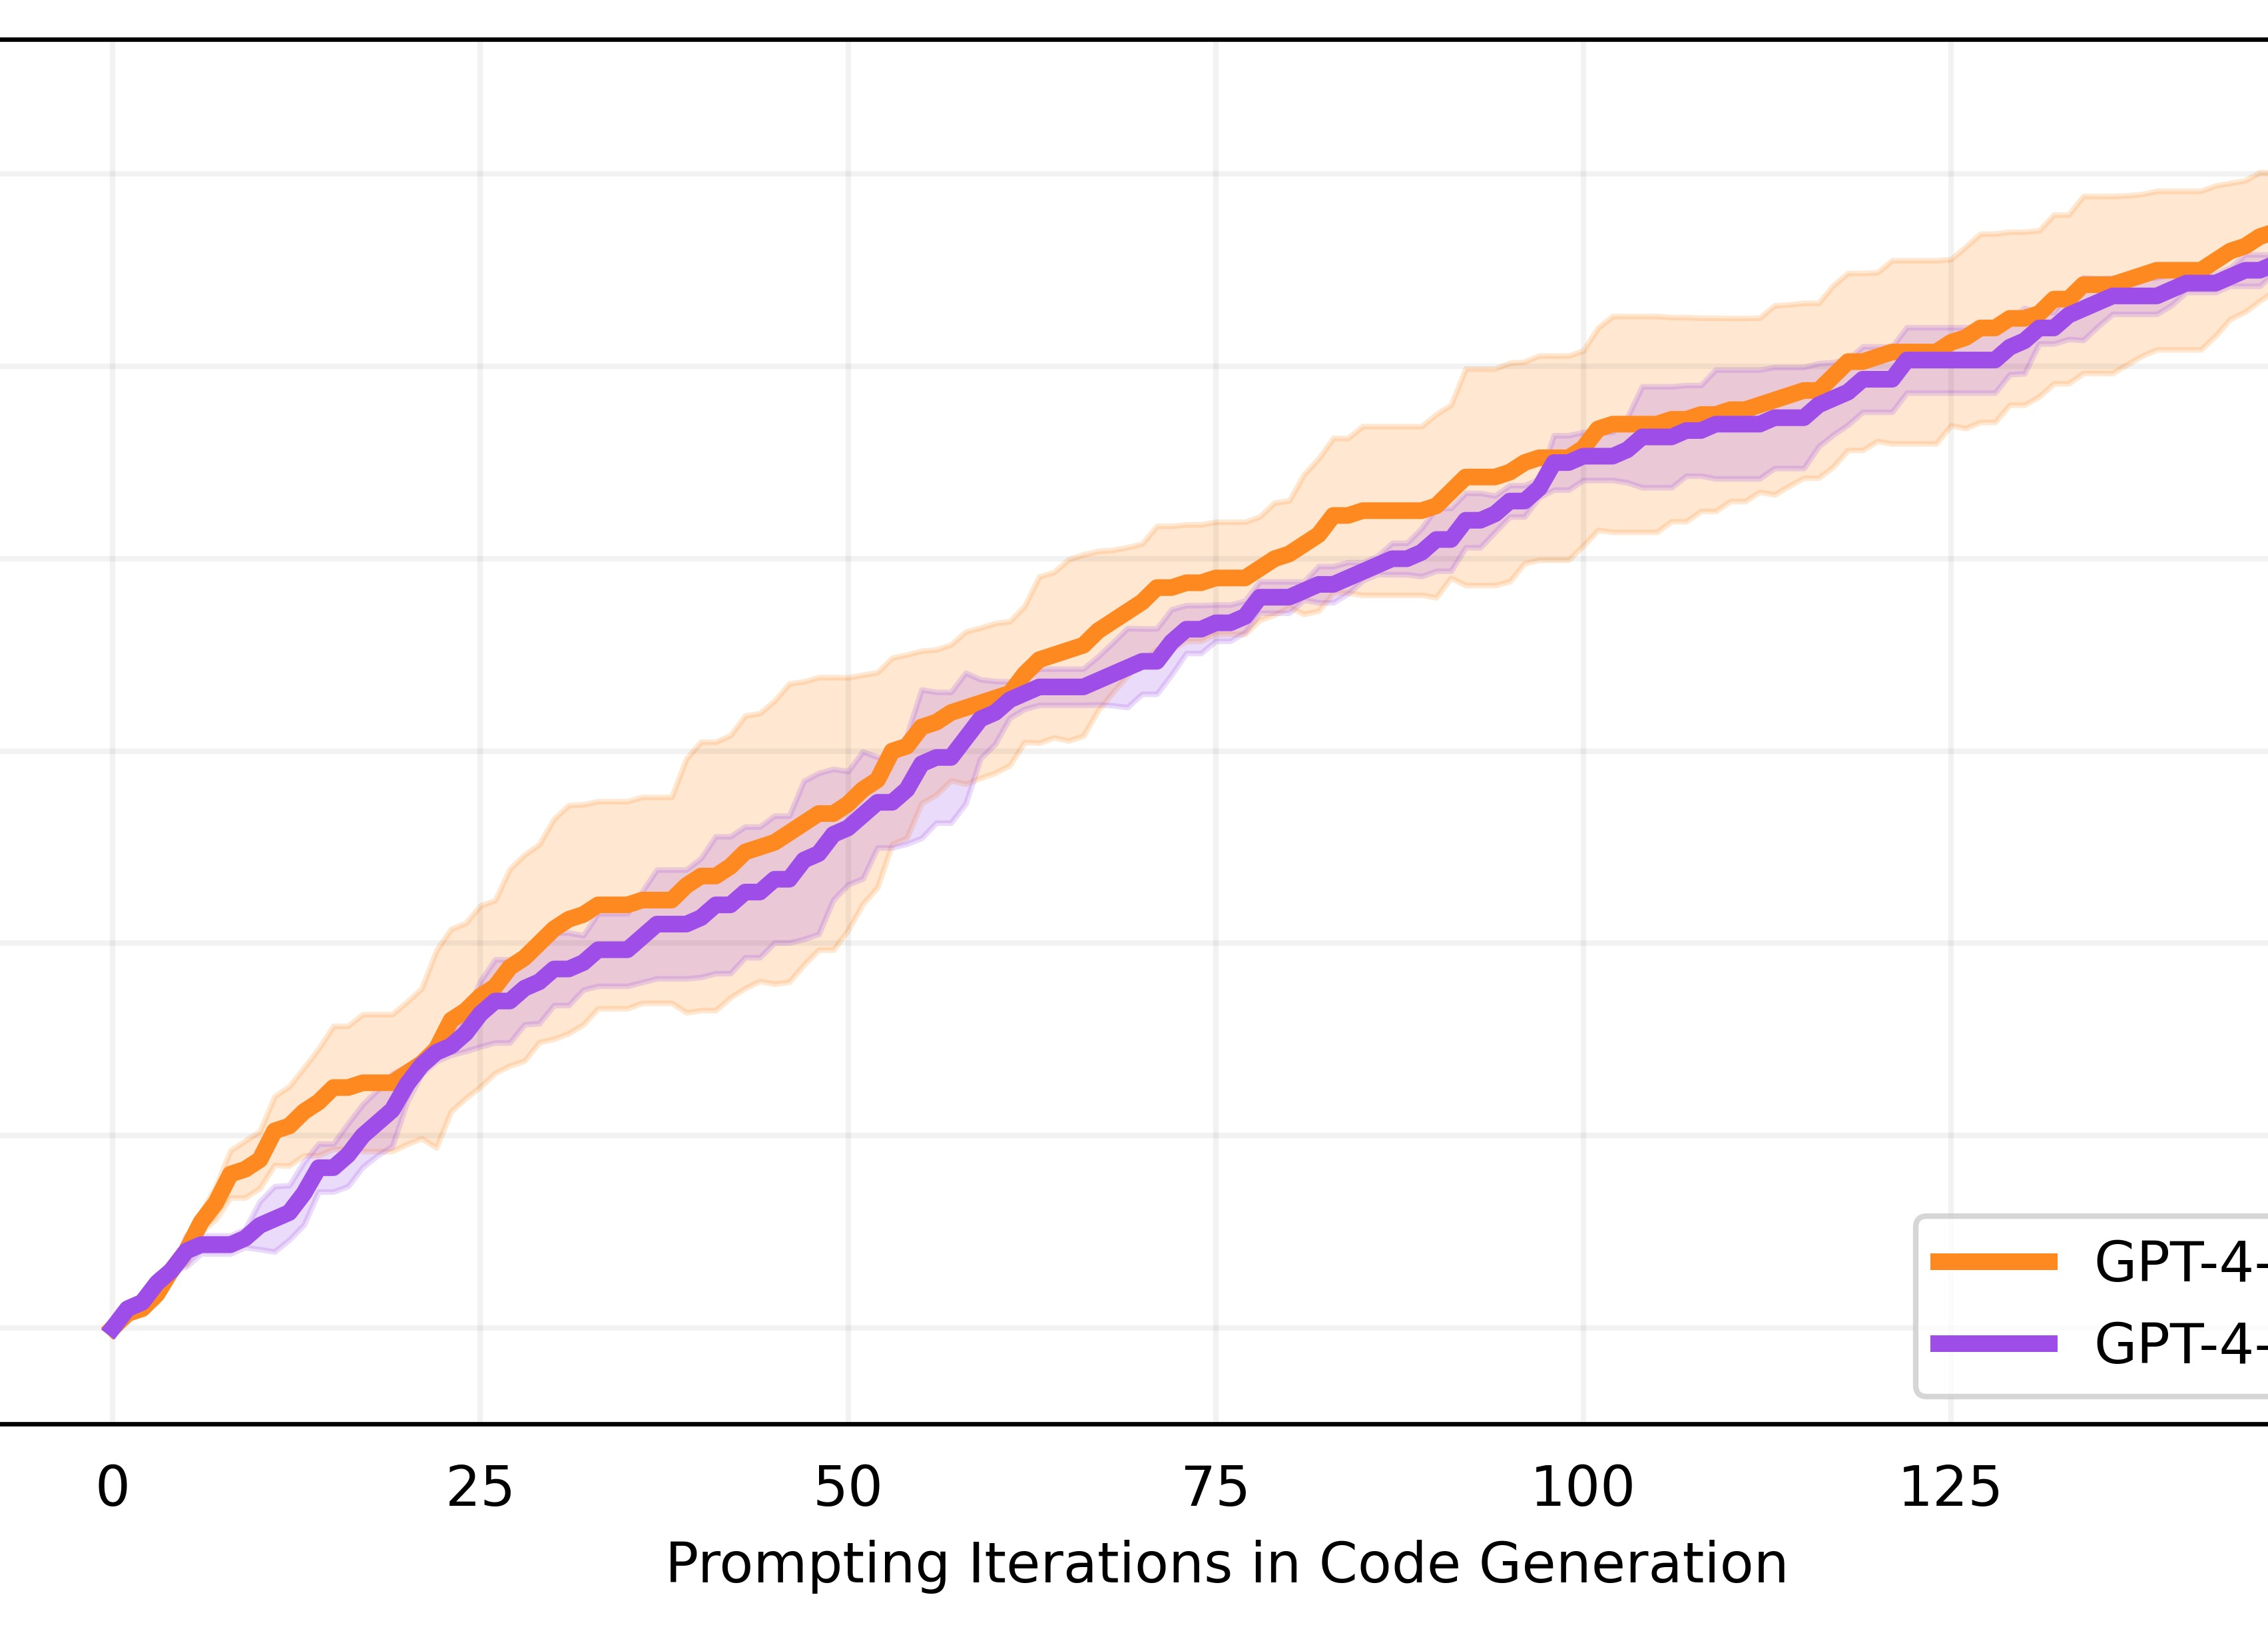
\includegraphics[width=1.891cm]{figures/img/canvas_tiles/plt_361.jpg}}};
\draw[black!35,line width=0.35pt] (7.916,-3.572) rectangle (9.807,-4.934);
\node[anchor=north west,text=ACMDarkBlue,font=\tiny\bfseries,inner sep=0] at (7.946,-4.964) {\href{https://arxiv.org/abs/2305.16291}{Voyager}};
\node[anchor=north west,text=black!60,font=\tiny,inner sep=0] at (7.946,-5.169) {\href{https://arxiv.org/abs/2305.16291}{Fig.\,A.4~p.42}};
\node[anchor=north west,inner sep=0] at (9.877,-3.572) {\href{https://arxiv.org/abs/1802.06070}{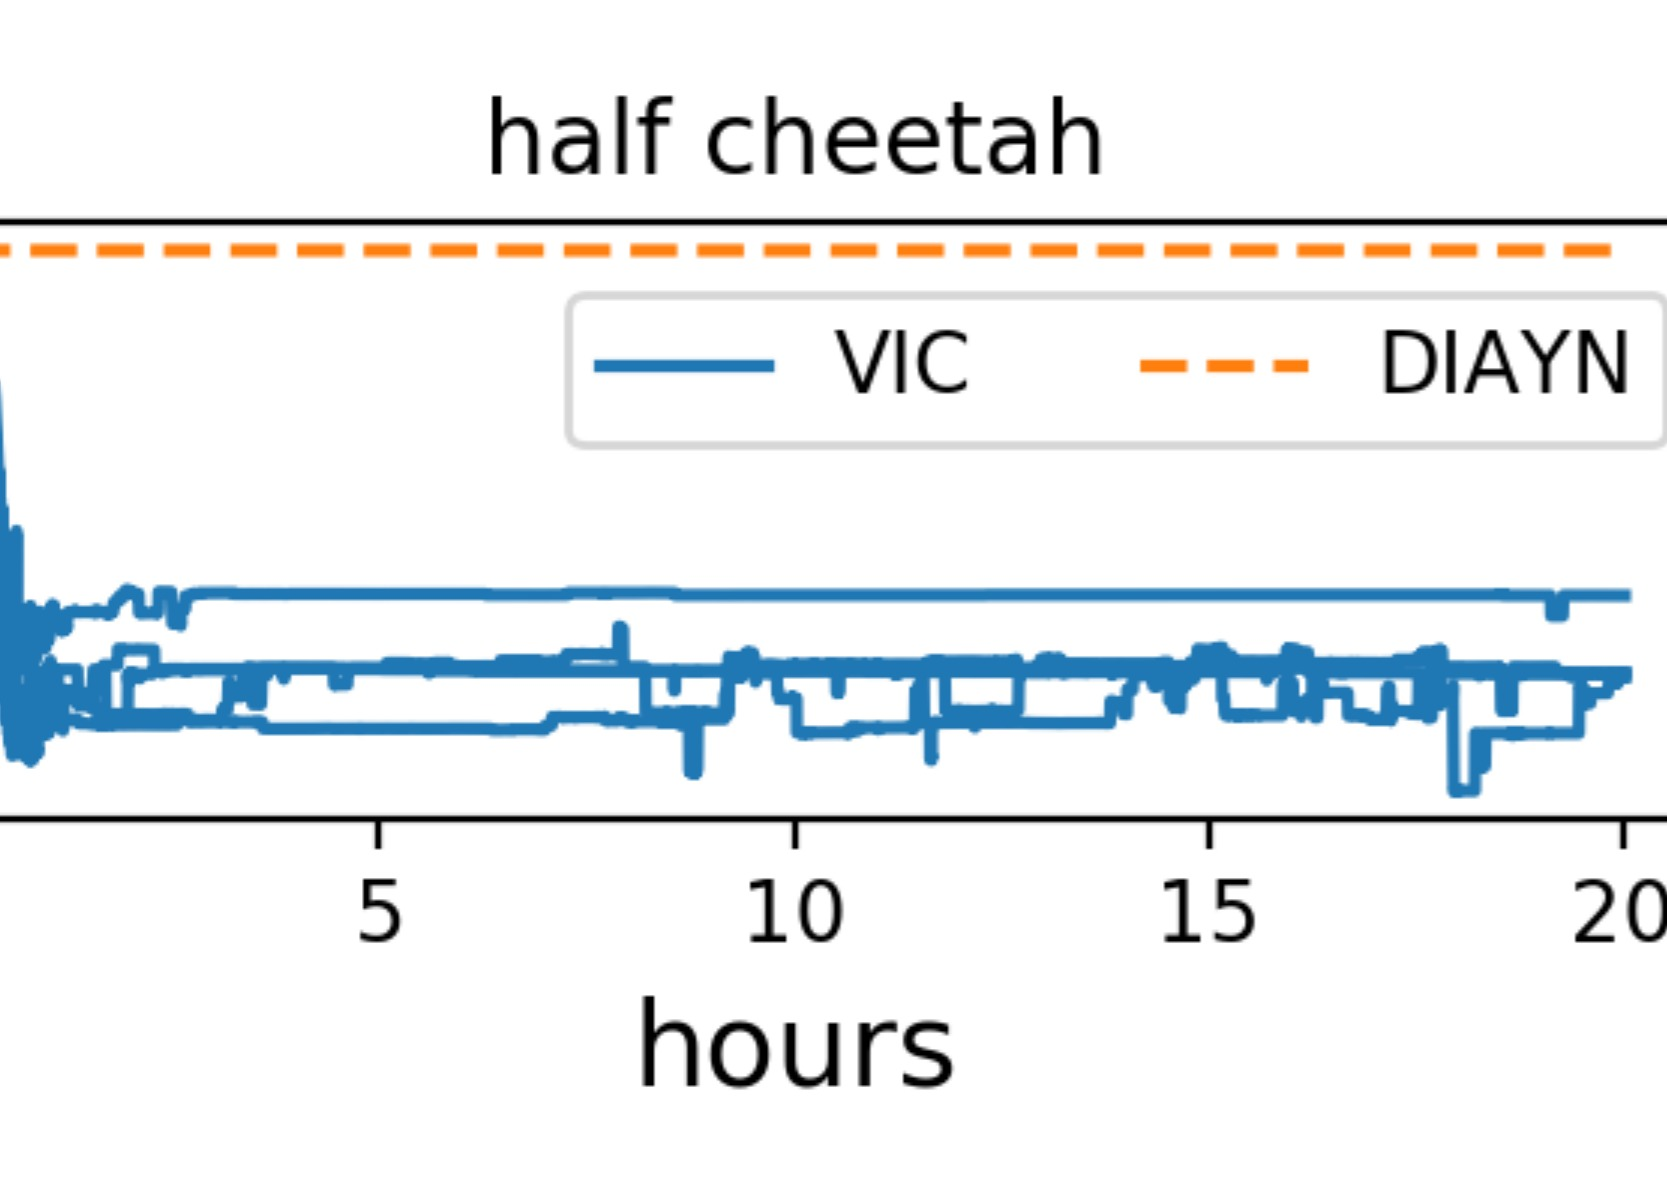
\includegraphics[width=1.891cm]{figures/img/canvas_tiles/plt_68.jpg}}};
\draw[black!35,line width=0.35pt] (9.877,-3.572) rectangle (11.769,-4.934);
\node[anchor=north west,text=ACMDarkBlue,font=\tiny\bfseries,inner sep=0] at (9.907,-4.964) {\href{https://arxiv.org/abs/1802.06070}{DIAYN}};
\node[anchor=north west,text=black!60,font=\tiny,inner sep=0] at (9.907,-5.169) {\href{https://arxiv.org/abs/1802.06070}{Fig.\,4~p.6}};
\node[anchor=north west,inner sep=0] at (11.839,-3.572) {\href{https://arxiv.org/abs/1907.01657}{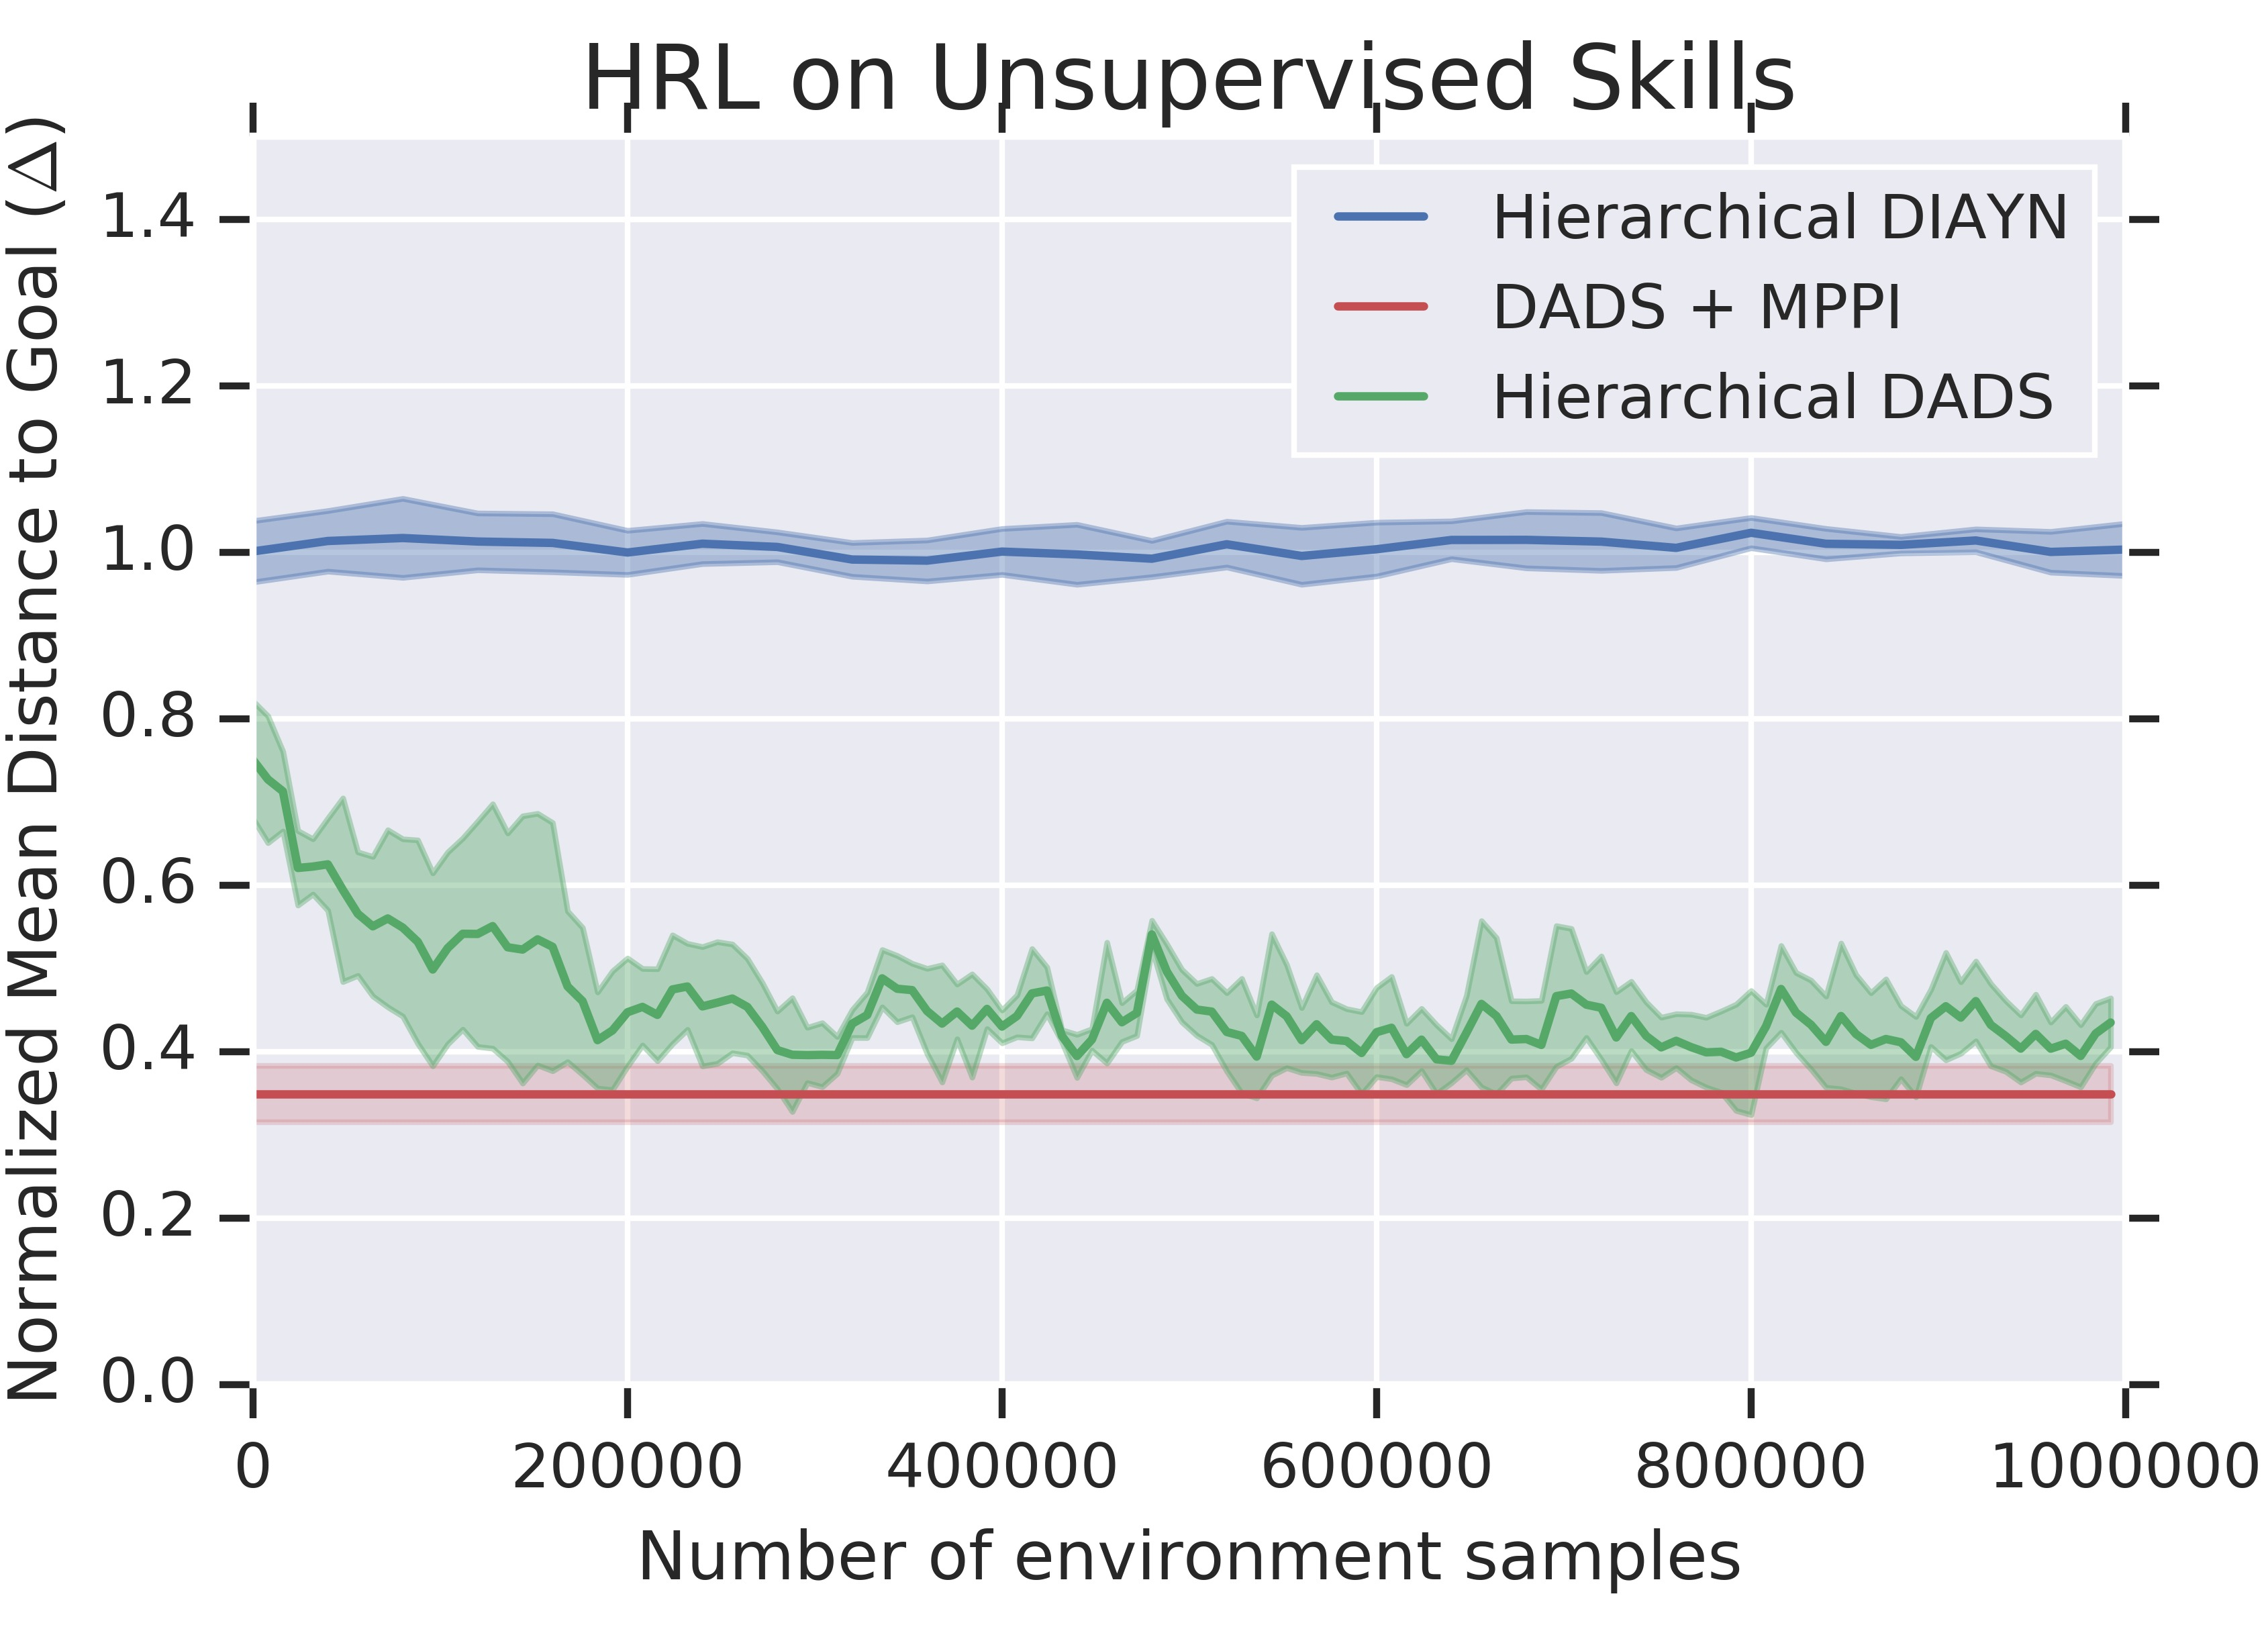
\includegraphics[width=1.891cm]{figures/img/canvas_tiles/plt_60.jpg}}};
\draw[black!35,line width=0.35pt] (11.839,-3.572) rectangle (13.730,-4.934);
\node[anchor=north west,text=ACMDarkBlue,font=\tiny\bfseries,inner sep=0] at (11.869,-4.964) {\href{https://arxiv.org/abs/1907.01657}{DADS}};
\node[anchor=north west,text=black!60,font=\tiny,inner sep=0] at (11.869,-5.169) {\href{https://arxiv.org/abs/1907.01657}{Fig.\,8~p.10}};
\fill[c5B3A8A] (0,-5.424) rectangle (13.800,-5.924);
\node[anchor=west,text=white,font=\footnotesize\bfseries,inner sep=0] at (0.14,-5.674) {Distributions, coverage and embeddings};
\node[anchor=north west,inner sep=0] at (1.051,-5.994) {\href{https://arxiv.org/abs/2410.24164}{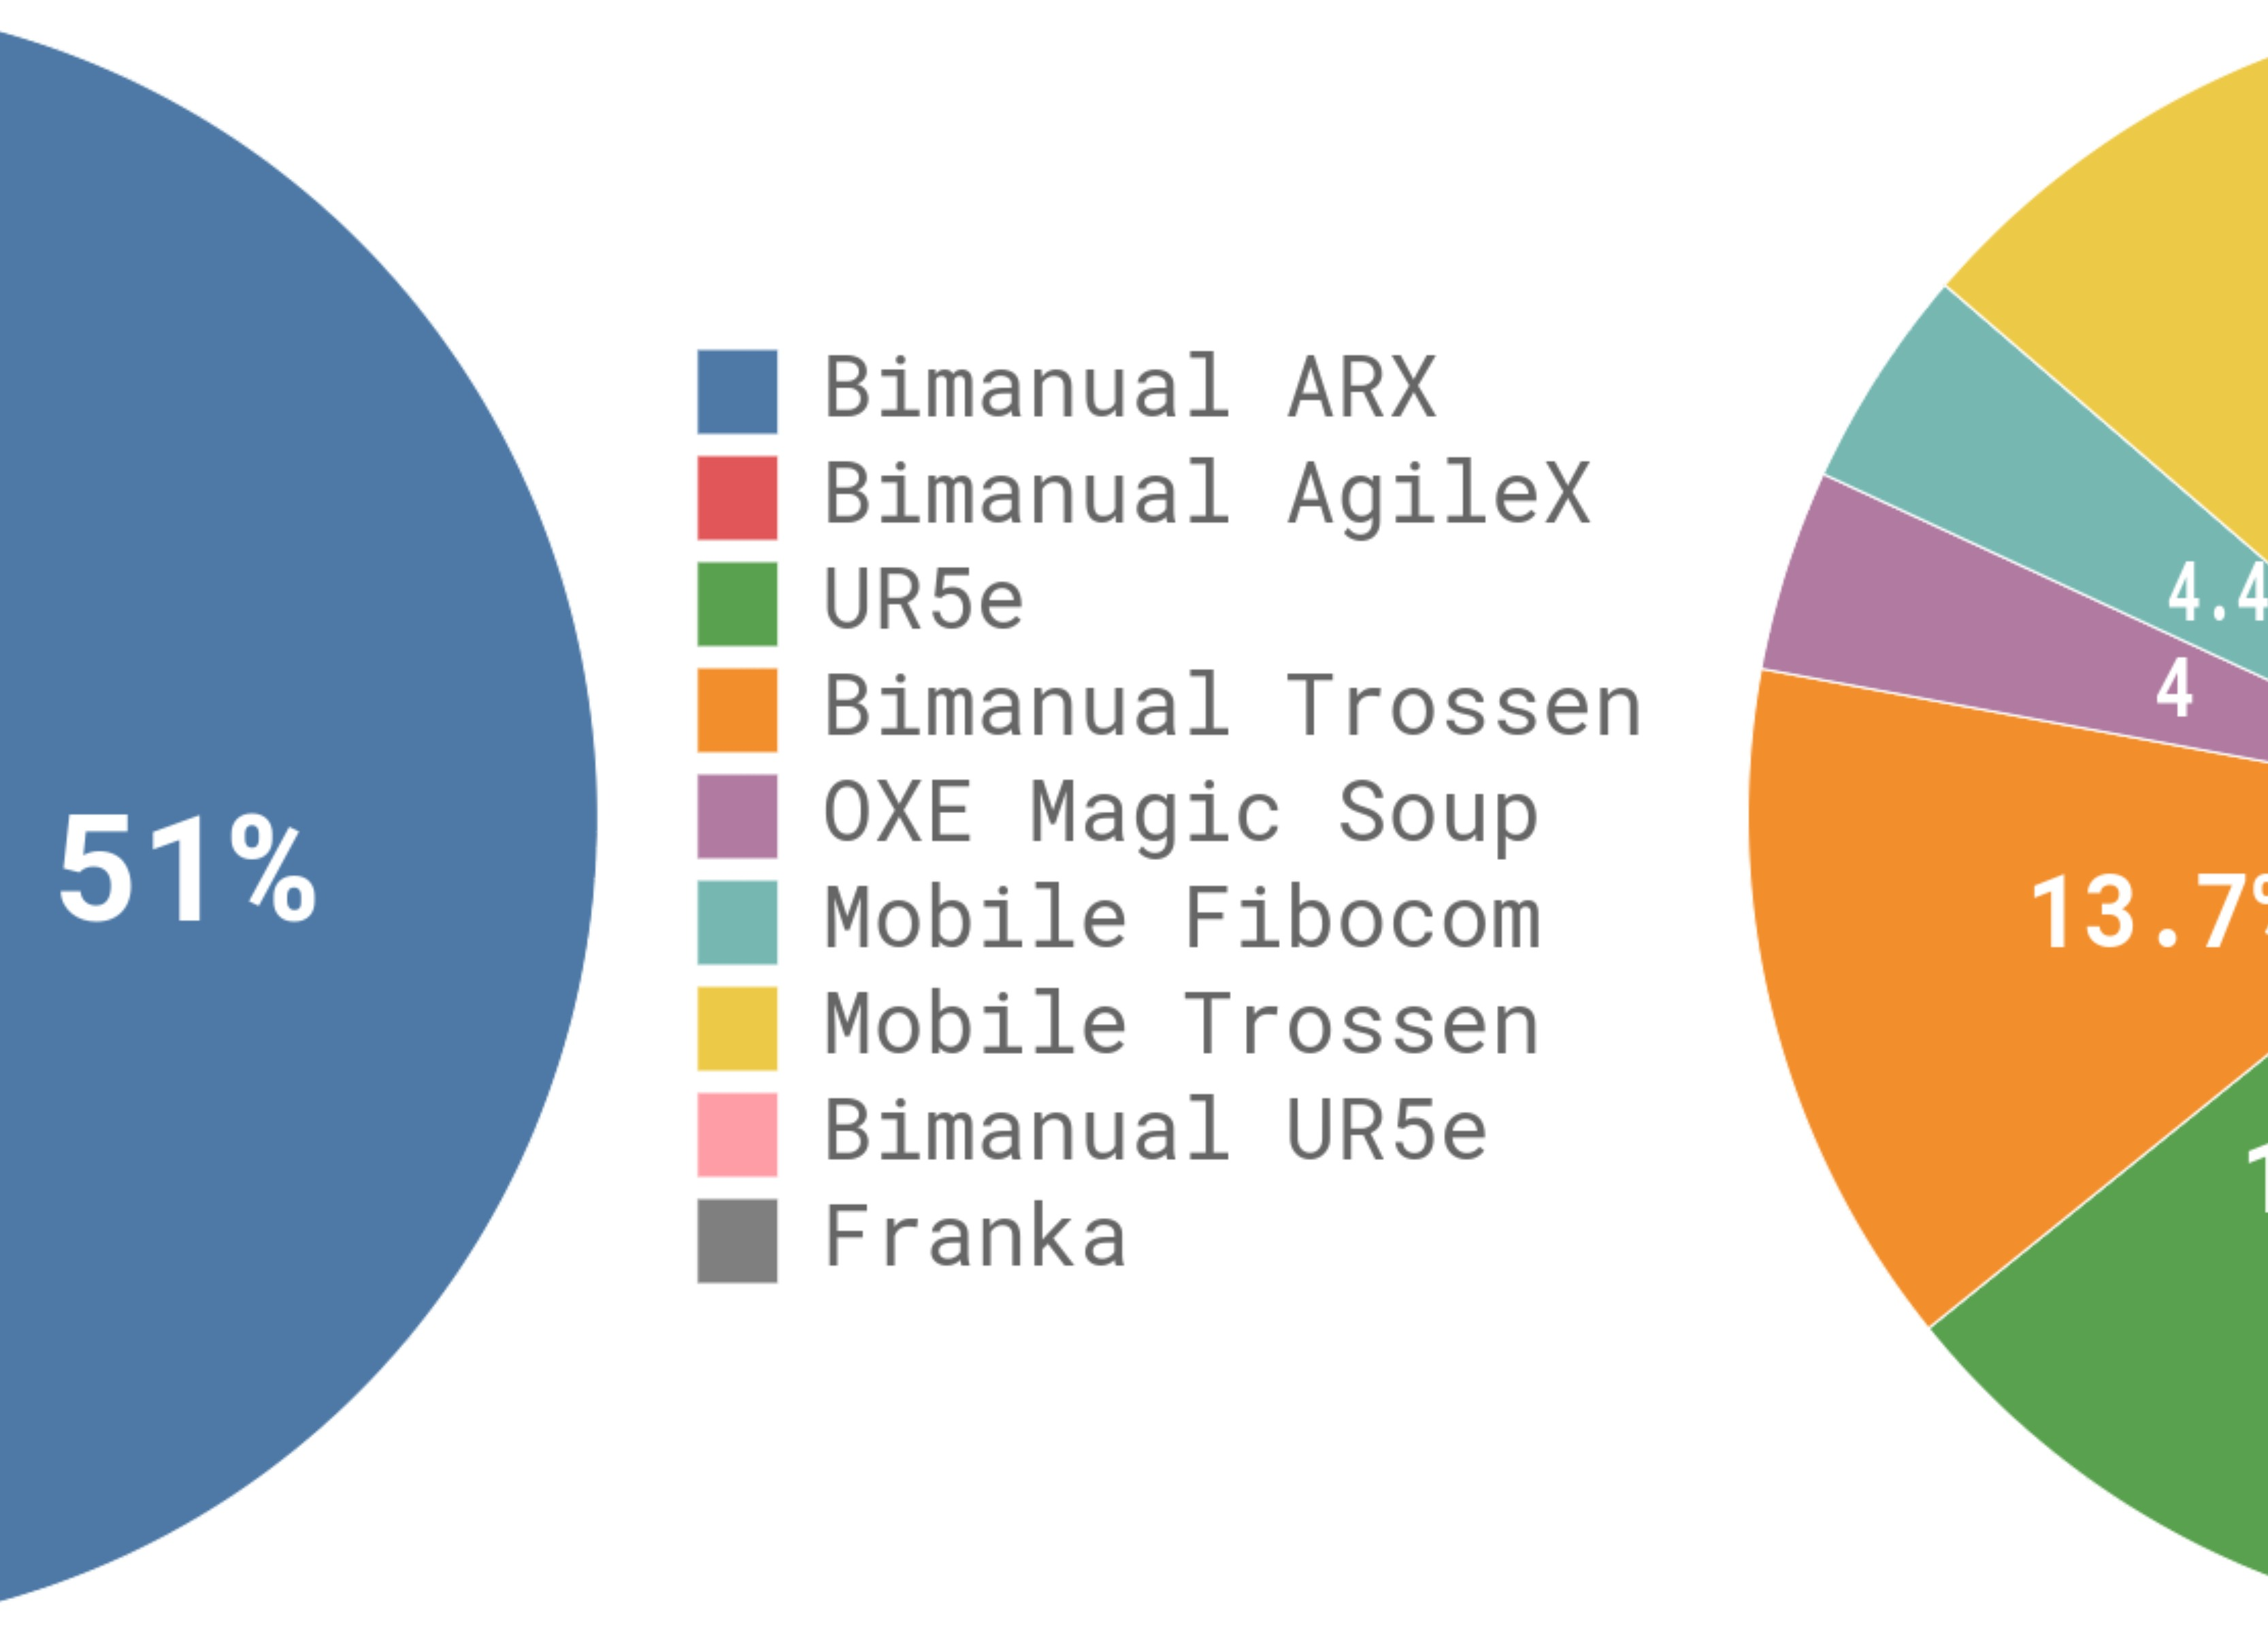
\includegraphics[width=1.891cm]{figures/img/canvas_tiles/plt_216.jpg}}};
\draw[black!35,line width=0.35pt] (1.051,-5.994) rectangle (2.942,-7.355);
\node[anchor=north west,text=ACMDarkBlue,font=\tiny\bfseries,inner sep=0] at (1.081,-7.385) {\href{https://arxiv.org/abs/2410.24164}{Pi-0}};
\node[anchor=north west,text=black!60,font=\tiny,inner sep=0] at (1.081,-7.590) {\href{https://arxiv.org/abs/2410.24164}{Fig.\,4~p.5}};
\node[anchor=north west,inner sep=0] at (3.012,-5.994) {\href{https://arxiv.org/abs/2207.07560}{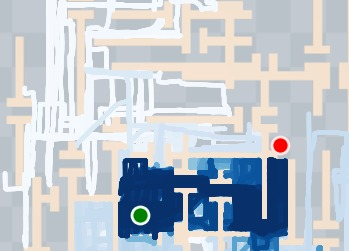
\includegraphics[width=1.891cm]{figures/img/canvas_tiles/plt_309.jpg}}};
\draw[black!35,line width=0.35pt] (3.012,-5.994) rectangle (4.904,-7.355);
\node[anchor=north west,text=ACMDarkBlue,font=\tiny\bfseries,inner sep=0] at (3.042,-7.385) {\href{https://arxiv.org/abs/2207.07560}{SkiMo}};
\node[anchor=north west,text=black!60,font=\tiny,inner sep=0] at (3.042,-7.590) {\href{https://arxiv.org/abs/2207.07560}{Fig.\,9~p.13}};
\node[anchor=north west,inner sep=0] at (4.974,-5.994) {\href{https://arxiv.org/abs/2010.13611}{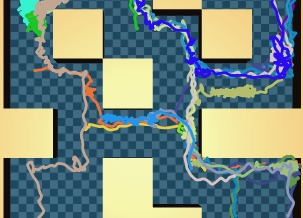
\includegraphics[width=1.891cm]{figures/img/canvas_tiles/plt_198.jpg}}};
\draw[black!35,line width=0.35pt] (4.974,-5.994) rectangle (6.865,-7.355);
\node[anchor=north west,text=ACMDarkBlue,font=\tiny\bfseries,inner sep=0] at (5.004,-7.385) {\href{https://arxiv.org/abs/2010.13611}{OPAL}};
\node[anchor=north west,text=black!60,font=\tiny,inner sep=0] at (5.004,-7.590) {\href{https://arxiv.org/abs/2010.13611}{Fig.\,1~p.2}};
\node[anchor=north west,inner sep=0] at (6.935,-5.994) {\href{https://arxiv.org/abs/2406.18746}{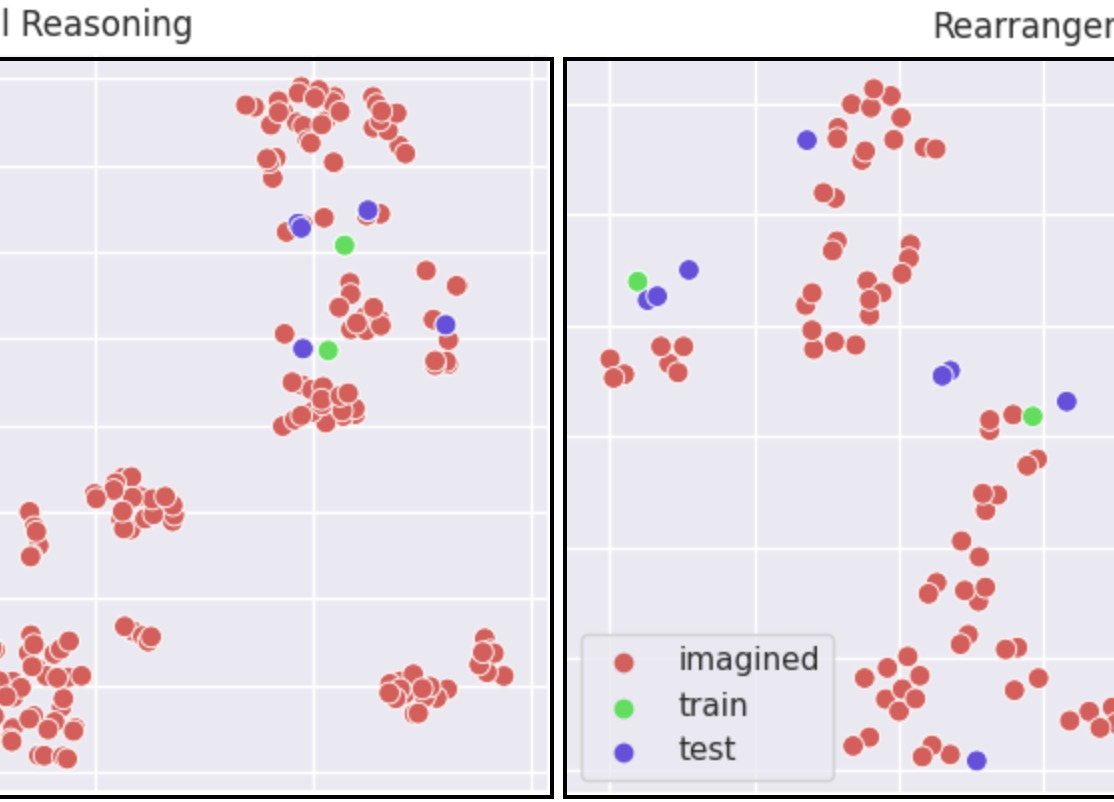
\includegraphics[width=1.891cm]{figures/img/canvas_tiles/plt_167.jpg}}};
\draw[black!35,line width=0.35pt] (6.935,-5.994) rectangle (8.826,-7.355);
\node[anchor=north west,text=ACMDarkBlue,font=\tiny\bfseries,inner sep=0] at (6.965,-7.385) {\href{https://arxiv.org/abs/2406.18746}{LRLL}};
\node[anchor=north west,text=black!60,font=\tiny,inner sep=0] at (6.965,-7.590) {\href{https://arxiv.org/abs/2406.18746}{Fig.\,3~p.6}};
\node[anchor=north west,inner sep=0] at (8.896,-5.994) {\href{https://arxiv.org/abs/2202.00914}{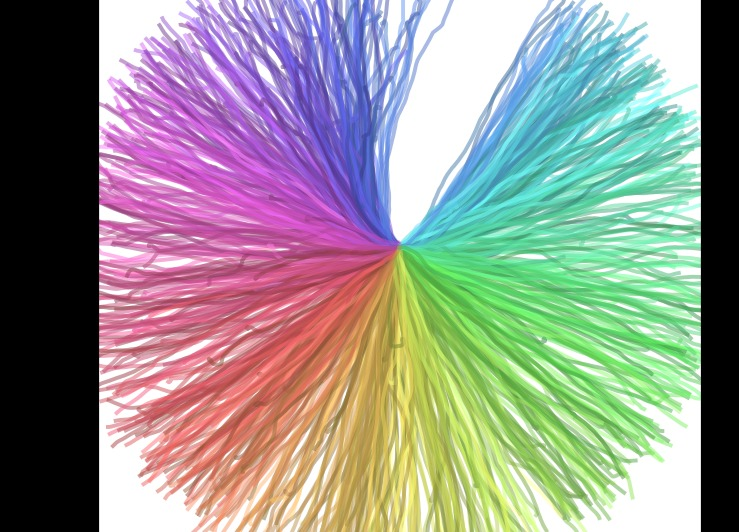
\includegraphics[width=1.891cm]{figures/img/canvas_tiles/plt_170.jpg}}};
\draw[black!35,line width=0.35pt] (8.896,-5.994) rectangle (10.788,-7.355);
\node[anchor=north west,text=ACMDarkBlue,font=\tiny\bfseries,inner sep=0] at (8.926,-7.385) {\href{https://arxiv.org/abs/2202.00914}{LSD}};
\node[anchor=north west,text=black!60,font=\tiny,inner sep=0] at (8.926,-7.590) {\href{https://arxiv.org/abs/2202.00914}{Fig.\,1b~p.2}};
\node[anchor=north west,inner sep=0] at (10.858,-5.994) {\href{https://arxiv.org/abs/2010.13611}{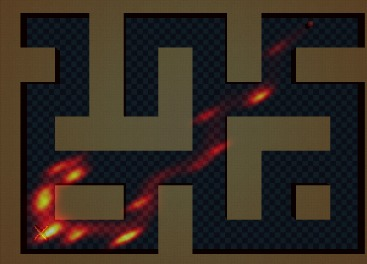
\includegraphics[width=1.891cm]{figures/img/canvas_tiles/plt_199.jpg}}};
\draw[black!35,line width=0.35pt] (10.858,-5.994) rectangle (12.749,-7.355);
\node[anchor=north west,text=ACMDarkBlue,font=\tiny\bfseries,inner sep=0] at (10.888,-7.385) {\href{https://arxiv.org/abs/2010.13611}{OPAL}};
\node[anchor=north west,text=black!60,font=\tiny,inner sep=0] at (10.888,-7.590) {\href{https://arxiv.org/abs/2010.13611}{Fig.\,3~p.8}};
\end{tikzpicture}}
\caption{\textbf{Results reported across the surveyed systems.} Representative results figures from the corpus, grouped into success-rate/ablation bars, training and scaling curves, and distribution, coverage and embedding plots. The results come from systems on both sides of the weights--skills axis (Figure~\ref{fig:corpus_collage}), grouped here by type of evidence. Each panel is a live hyperlink to the source paper on arXiv and is annotated with the exact figure number it was cropped from (also in Table~\ref{tab:canvas_provenance}). Panels convey the shape and variety of empirical evidence, not absolute comparisons across incommensurable protocols. Images \textcopyright\ their respective authors, reproduced for scholarly review.}
\Description{A labelled grid of results charts in three bands: success-rate and ablation bar charts, training and scaling curves, and distribution/coverage/embedding plots; each tile is a hyperlink labelled with its system name and source figure number.}
\label{fig:plots_canvas}
\end{figure*}
